\section{Parahoric restriction tables}
Let us clarify some of the notation used in the tables below. We use the notation described in \ref{notation:Langlandsparam} for the Langlands labels parametrizing the unipotent representations of $G=F_4(F)$. This is the same notation used in Reeder's tables \cite{Reeder2000}. The unipotent representations of finite reductive groups of Lie type are labelled as follows. For groups of type $A_n$, they are parametrized by partitions $\lambda$ of $n+1$. For groups of type $B_n/C_n$, the principal series representations are parametrized by double partitions $[\lambda,\mu]$ of $n$. To understand these tables, it is enough to know that groups of type $B_3/C_3$ have two non-principal series representations $\theta_1$ and $\theta_2$, while groups of type $B_4/C_4$ have five non-principal series representations $\theta_1,\ldots,\theta_5$. They all lie in the same representation series, arising from the unipotent cuspidal representation of their Levi subgroup of type $B_2/C_2$.

A finite group of Lie type of type $A_1$ has only two unipotent characters; the trivial and the Steinberg. Whenever the type of reductive quotient is the product of two simple types, one of which is $A_1$, we give the multiplicities for each character $\chi$ of the other type as a pair $a,\overline{b}$, where $a$ and $\overline{b}$ are the multiplicities of $\chi\otimes\mathbf{1}_{A_1}$ and $\chi\otimes\St_{A_1}$, respectively.

\subsection{Parahoric restriction tables for \texorpdfstring{$F_4$}{PDFstring}}
For every parahoric subgroup $K_i,i\in\{1,2,3,4\}$, we present two tables. The first one is the table of parahoric restrictions for all Iwahori-spherical representations of $F_4(F)$ of interest. The second table contains the parahoric restrictions of all virtual characters $\Pi(u,s,h)$, where representations of $\overline{K}_i$ are organized in terms of the families. Firstly, we write the characters in trivial families; then we write each family, with the special character always coming first. We omit the tables for the maximal hyperspecial parahoric subgroup $K_0$, for the restrictions can be found in \cite{Reeder2000}[\S 10], and the conjecture has already been verified in \cite{Ciubotaru2020}. In particular, all nontrivial families $\mathcal{U}$ that appear in the tables have size $4$, with corresponding group $\Gamma_\mathcal{U}=C_2$, so Lusztig's non-abelian Fourier transform acts by 
$$\begin{pmatrix}
    \frac{1}{2} & \frac{1}{2} & \frac{1}{2} & \frac{1}{2} \\
    \frac{1}{2} & \frac{1}{2} & -\frac{1}{2} & -\frac{1}{2} \\
    \frac{1}{2} & -\frac{1}{2} & \frac{1}{2} & -\frac{1}{2} \\
    \frac{1}{2} & -\frac{1}{2} & -\frac{1}{2} & \frac{1}{2} 
\end{pmatrix}.$$

From these tables, the statement of Theorem \ref{thm:F4} can be easily verified using Lusztig's nonabelian transform. For reference, we write here the virtual characters $\Pi(u,s,h)$ in terms of representations of $F_4(F)$ when $u\in F_4(a_3)$. In the notation below, $\tau=g_2\cdot g_2'$ is another $2$-cycle conjugate to $g_2$ in $A_u=S_4$ but not in $A_{ug_2}=C_2\times C_2$ and, similarly, $\gamma$ is an element conjugate to $g_2'$ in $A_u=S_4$ but not in $A_{ug_2'}=D_8$. The analogous expressions for other unipotent classes are much simpler. 

\begin{align*}
    \Pi(F_4(a_3), 1, 1)&= [F_4(a_3),4] + 3[F_4(a_3),31] + 3[F_4(a_3),211] + [F_4(a_3),1^4] + 2[F_4(a_3),22]; \\
    \Pi(F_4(a_3), 1, g_2) &= [F_4(a_3),4] + [F_4(a_3),31] - [F_4(a_3),211] - [F_4(a_3),1^4]; \\
    \Pi(F_4(a_3), 1, g_2') &= [F_4(a_3),4] - [F_4(a_3),31] - [F_4(a_3),211] + [F_4(a_3),1^4] + 2[F_4(a_3),22]; \\
    \Pi(F_4(a_3), 1, g_3) &= [F_4(a_3),4] + [F_4(a_3),1^4] - [F_4(a_3),22]; \\
    \Pi(F_4(a_3), 1, g_4) &= [F_4(a_3),4] - [F_4(a_3),31] + [F_4(a_3),211] - [F_4(a_3),1^4]; 
\end{align*}
\begin{align*}
    \Pi(F_4(a_3), g_2, 1) &= [C(42)A_1,++] + [C(42)A_1,+-] + [C(42)A_1,-+] + [C(42)A_1,--]; \\
    \Pi(F_4(a_3), g_2, g_2) &= [C(42)A_1,++] - [C(42)A_1,+-] + [C(42)A_1,-+] - [C(42)A_1,--]; \\
    \Pi(F_4(a_3), g_2, \tau) &= [C(42)A_1,++] + [C(42)A_1,+-] - [C(42)A_1,-+] - [C(42)A_1,--]; \\
    \Pi(F_4(a_3), g_2, g_2') &= [C(42)A_1,++] - [C(42)A_1,+-] - [C(42)A_1,-+] + [C(42)A_1,--]; 
\end{align*}
\begin{align*}
    \Pi(F_4(a_3), g_2',1) &= [B_4(531),\mathbf{1}] + 2[B_4(531),r] + [B_4(531),\varepsilon'] + [B_4(531),\varepsilon''] + [B_4(531),\varepsilon]; \\
    \Pi(F_4(a_3), g_2', g_2') &= [B_4(531),\mathbf{1}] - [B_4(531),\varepsilon'] + [B_4(531),\varepsilon''] - [B_4(531),\varepsilon]; \\
    \Pi(F_4(a_3), g_2', g_2'') &= [B_4(531),\mathbf{1}] - 2[B_4(531),r] + [B_4(531),\varepsilon'] + [B_4(531),\varepsilon''] + [B_4(531),\varepsilon]; \\
    \Pi(F_4(a_3), g_2', g_4) &= [B_4(531),\mathbf{1}] - [B_4(531),\varepsilon'] - [B_4(531),\varepsilon''] + [B_4(531),\varepsilon]; \\
    \Pi(F_4(a_3), g_2', \gamma) &= [B_4(531),\mathbf{1}] + [B_4(531),\varepsilon'] - [B_4(531),\varepsilon''] - [B_4(531),\varepsilon];
\end{align*}
\begin{align*}
    \Pi(F_4(a_3), g_3, 1) &= [2A_2,\mathbf{1}] + [2A_2,\theta] + [2A_2,\theta^2]; \\
    \Pi(F_4(a_3), g_3, g_3) &= [2A_2,\mathbf{1}] + \theta^2[2A_2,\theta] + \theta[2A_2,\theta^2]; \\
    \Pi(F_4(a_3), g_3, g_3^{-1}) &= [2A_2,\mathbf{1}] + \theta[2A_2,\theta] + \theta^2[2A_2,\theta^2];
\end{align*}
\begin{align*}
    \Pi(F_4(a_3), g_4, 1) &= [A_3A_1,1] + [A_3A_1,i] + [A_3A_1,-1] + [A_3A_1,-i]; \\
    \Pi(F_4(a_3), g_4, g_4) &= [A_3A_1,1] - i[A_3A_1,i] - [A_3A_1,-1] - i[A_3A_1,-i]; \\
    \Pi(F_4(a_3), g_4, g_4') &= [A_3A_1,1] - [A_3A_1,i] + [A_3A_1,-1] - [A_3A_1,-i]; \\
    \Pi(F_4(a_3), g_4, g_4^{-1}) &= [A_3A_1,1] + i[A_3A_1,i] - [A_3A_1,-1] - i[A_3A_1,-i];
\end{align*}

\iffalse
\newpage
\begin{align*}
    \Pi(E_6,1,1)&=[E_6,1];\\
    \Pi(E_6(a_1),1,1)&=[E_6(a_1),1];\\
    \Pi(E_6(a_3),1,1)&=[E_6(a_3),+]+[E_6(a_3),-];\\
    \Pi(E_6(a_3),1,g_2)&=[E_6(a_3),+]-[E_6(a_3),-];\\
    \Pi(E_6(a_3),g_2,1)&=[A_1A_5,+]+[A_1A_5,-];\\
    \Pi(E_6(a_3),g_2,g_2)&=[A_1A_5,+]-[A_1A_5,-];\\
    \Pi(D_4,s_3,w_3)&=[D_4(71),1]+\theta[D_4(71),\theta]+\theta^2[D_4(71),\theta^2];\\
    \Pi(D_4,s_3,w_3^{-1})&=[D_4(71),1]+\theta^2[D_4(71),\theta]+\theta[D_4(71),\theta^2];\\
    \Pi(D_4(a_1),1,g_3)&=[D_4(a_1),1]+[D_4(a_1),\varepsilon]-[D_4(a_1),r];\\
    \Pi(D_4(a_1),z,g_3)&=[D_4(53),\mathbf{1}]+\theta[D_4(53),\theta]+\theta^2[D_4(53),\theta^2];\\
    \Pi(D_4(a_1),z^2,g_3)=\Pi(D_4(a_1),z,g_3^{-1})&=[D_4(53),\mathbf{1}]+\theta^2[D_4(53),\theta]+\theta[D_4(53),\theta^2];\\
    \Pi(D_4(a_1),g_3,1)&=[3A_2,\mathbf{1}]+[3A_2,\theta]+[3A_2,\theta];\\
    \Pi(D_4(a_1),g_3,z)&=[3A_2,\mathbf{1}]+\theta[3A_2,\theta]+\theta^2[3A_2,\theta];\\
    \Pi(D_4(a_1),g_3,z^2)&=[3A_2,\mathbf{1}]+\theta^2[3A_2,\theta]+\theta[3A_2,\theta];\\
    \Pi(A_2,s_{3,3},w_{3,3})=\Pi(A_2,s_{3,3},w_{3,3}^2)&=[D_4(3311),\mathbf{1}]+[D_4(3311),\epsilon];\\
\end{align*}
\fi
\newpage




\begin{landscape}
    \centering
    \subsubsection*{Iwahori-spherical \texorpdfstring{$B_4$}{PDFstring}-types}
    \begin{table}[ht]
        \centering
        {\small
        \begin{tabular}{|c|cccccccccccc|}
            \hline
            & $[21^2,\cdot]$ & $[1^4,\cdot]$ & $[1^3,1]$ & $[2,11]$ & $[11,2]$ & $[11,11]$ & $[1,21]$ & $[1,1^3]$ & $[\cdot,31]$ & $[\cdot,22]$ & $[\cdot,21^2]$ & $[\cdot,1^4]$ \\\hline
            $[F_4,1]$ & 0 & 0 & 0 & 0 & 0 & 0 & 0 & 0 & 0 & 0 & 0 & 1\\\hline
            $[F_4(a_1),+]$ & 0 & 0 & 0 & 0 & 0 & 0 & 0 & 1 & 0 & 0 & 0 & 1\\
            $[F_4(a_1),-]$ & 0 & 1 & 0 & 0 & 0 & 0 & 0 & 0 & 0 & 0 & 0 & 1\\
            $[B_4,+]$ & 0 & 0 & 0 & 0 & 0 & 0 & 0 & 0 & 0 & 0 & 1 & 0\\\hline
            $[F_4(a_2),+]$ & 0 & 0 & 0 & 0 & 0 & 1 & 0 & 1 & 0 & 0 & 1 & 1\\
            $[F_4(a_2),-]$ & 0 & 0 & 0 & 0 & 0 & 0 & 0 & 0 & 0 & 1 & 0 & 0\\
            $[C_3A_1,+]$ & 0 & 0 & 1 & 0 & 0 & 0 & 0 & 1 & 0 & 0 & 1 & 1\\\hline
            $[B_4(711),+]$ & 0 & 0 & 0 & 0 & 0 & 0 & 1 & 1 & 0 & 0 & 1 & 0\\
            $[B_4(711),-]$ & 0 & 0 & 0 & 0 & 0 & 1 & 0 & 0 & 0 & 1 & 0 & 1\\\hline
            $[F_4(a_3),4]$ & 0 & 0 & 1 & 1 & 1 & 1 & 1 & 2 & 0 & 0 & 1 & 1\\
            $[F_4(a_3),31]$ & 1 & 1 & 1 & 0 & 0 & 1 & 0 & 1 & 0 & 0 & 0 & 1 \\
            $[F_4(a_3),22]$ & 0 & 0 & 0 & 1 & 0 & 0 & 0 & 1 & 0 & 0 & 0 & 0 \\
            $[F_4(a_3),211]$ & 0 & 1 & 0 & 0 & 0 & 0 & 0 & 0 & 0 & 0 & 0 & 0 \\
            $[C_3(42)A_1,++]$ & 1 & 0 & 1 & 1 & 1 & 1 & 1 & 2 & 0 & 0 & 2 & 1 \\
            $[C_3(42)A_1,+-]$ & 0 & 1 & 1 & 0 & 0 & 1 & 0 & 0 & 0 & 0 & 0 & 1 \\
            $[B_4(531),1]$ & 0 & 0 & 0 & 1 & 1 & 0 & 1 & 1 & 1 & 0 & 2 & 0 \\
            $[B_4(531),\varepsilon']$ & 0 & 0 & 0 & 0 & 0 & 0 & 0 & 0 & 1 & 0 & 0 & 0 \\
            $[B_4(531),\varepsilon'']$ & 1 & 0 & 0 & 0 & 0 & 0 & 0 & 0 & 0 & 0 & 1 & 0 \\
            $[2A_2,1]$ & 0 & 0 & 1 & 0 & 1 & 1 & 1 & 1 & 0 & 0 & 1 & 1 \\
            $[A_1A_3,1]$ & 0 & 0 & 0 & 0 & 1 & 0 & 1 & 1 & 1 & 0 & 1 & 0 \\\hline
        \end{tabular}
        }
        \caption{Parahoric restriction of unipotent $F_4(F)$-representations with respect to $K_1$}
    \end{table}
    \iffalse
    \begin{table}[ht]
        \centering
        {\tiny
        \begin{tabular}{|c|ccccc|cccR|cccR|cccR|cccR|}
            \hline
        & $[4,\cdot]$ & $[21,1]$ & $[11,2]$ & $[1,21]$ & $[\cdot,1^4]$ & $[1,1^3]$ & $[1^4,\cdot]$ & $[\cdot,21^2]$ & $\theta_1$ & $[11,11]$ & $[1^3,1]$ & $[\cdot,22]$ & $\theta_2$ & $[2,11]$ & $[21^2,\cdot]$ & $[\cdot,31]$ & $\theta_3$ & $[2,2]$ & $[22,\cdot]$ & $[1,3]$ & $\theta_4$ \\\hline
        $\Pi(u,1,1)$ & 0 & 0 & 1 & 1 & 4 & 7 & 6 & 1 & 0 & 4 & 4 & 0 & 0 & 3 & 3 & 0 & 0 & 0 & 0 & 0 & 0 \\
        $\Pi(u,1,g_2)$ & 0 & 0 & 1 & 1 & 2 & 3 & 0 & 1 & 0 & 2 & 2 & 0 & 0 & 1 & 1 & 0 & 0 & 0 & 0 & 0 & 0 \\
        $\Pi(u,1,g_2')$ & 0 & 0 & 1 & 1 & 0 & 3 & -2 & 1 & 0 & 0 & 0 & 0 & 0 & 3 & -1 & 0 & 0 & 0 & 0 & 0 & 0 \\
        $\Pi(u,1,g_3)$ & 0 & 0 & 1 & 1 & 1 & 1 & 0 & 1 & 0 & 1 & 1 & 0 & 0 & 0 & 0 & 0 & 0 & 0 & 0 & 0 & 0 \\
        $\Pi(u,1,g_4)$ & 0 & 0 & 1 & 1 & 0 & 1 & 0 & 1 & 0 & 0 & 0 & 0 & 0 & 1 & -1 & 0 & 0 & 0 & 0 & 0 & 0 \\\hline
        $\Pi(u,g_2,1)$  & 0 & 0 & 1 & 1 & 2 & 2 & 1 & 2 & 1 & 2 & 2 & 0 & 0 & 1 & 1 & 0 & 0 & 0 & 0 & 0 & 0 \\
        $\Pi(u,g_2,g_2)$ & 0 & 0 & 1 & 1 & 2 & 2 & 1 & 2 & {-1} & 2 & 2 & 0 & 0 & 1 & 1 & 0 & 0 & 0 & 0 & 0 & 0 \\
        $\Pi(u,g_2,\tau)$ & 0 & 0 & 1 & 1 & 0 & 2 & {-1} & 2 & 1 & 0 & 0 & 0 & 0 & 1 & 1 & 0 & 0 & 0 & 0 & 0 & 0 \\
        $\Pi(u,g_2,g_2')$ & 0 & 0 & 1 & 1 & 0 & 2 & {-1} & 2 & {-1} & 0 & 0 & 0 & 0 & 1 & 1 & 0 & 0 & 0 & 0 & 0 & 0 \\\hline
        $\Pi(u,g_2',1)$ & 0 & 0 & 1 & 1 & 0 & 1 & 0 & {3} & 2 & 0 & 0 & 0 & 0 & 1 & 1 & 2 & 2 & 0 & 0 & 0 & 0 \\
        $\Pi(u,g_2',g_2)$ &  0 & 0 & 1 & 1 & 0 & 1 & 0 & {3} & 0 & 0 & 0 & 0 & 0 & 1 & 1 & 0 & 0 & 0 & 0 & 0 & 0 \\
        $\Pi(u,g_2',g_2')$ & 0 & 0 & 1 & 1 & 0 & 1 & 0 & {3} & {-2} & 0 & 0 & 0 & 0 & 1 & 1 & 2 & {-2} & 0 & 0 & 0 & 0 \\
        $\Pi(u,g_2',\gamma)$ & 0 & 0 & 1 & 1 & 0 & 1 & 0 & 1 & 0 & 0 & 0 & 0 & 0 & 1 & {-1} & 2 & 0 & 0 & 0 & 0 & 0 \\
        $\Pi(u,g_2',g_4)$ & 0 & 0 & 1 & 1 & 0 & 1 & 0 & 1 & 0 & 0 & 0 & 0 & 0 & 1 & {-1} & 0 & 0 & 0 & 0 & 0 & 0 \\\hline
        $\Pi(u,g_3,h)$ & 0 & 0 & 1 & 1 & 1 & 1 & 0 & 1 & 0 & 1 & 1 & 0 & 0 & 0 & 0 & 0 & 0 & 0 & 0 & 0 & 0 \\\hline
        $\Pi(u,g_4,1/g_2')$ & 0 & 0 & 1 & 1 & 0 & 1 & 0 & 1 & 0 & 0 & 0 & 0 & 0 & 0 & 0 & 1 & 1 & 0 & 0 & 0 & 0 \\
        $\Pi(u,g_4,g_4^{\pm1})$ & 0 & 0 & 1 & 1 & 0 & 1 & 0 & 1 & 0 & 0 & 0 & 0 & 0 & 0 & 0 & 1 & {-1} & 0 & 0 & 0 & 0 \\\hline
        \end{tabular}
        }
        \caption{Parahoric restrictions of the virtual characters $\Pi(u,s,h)$ where $u\in F_4(a_3)$ with respect to $K_1$}
    \end{table}
    \fi

    \newpage

    \begin{table}[ht]
        \centering
        {\small
        \begin{tabular}{|c|ccc|cccc|cccc|cccc|}
            \hline
            & $[11,2]$ & $[1,21]$ & $[\cdot,1^4]$ & $[1,1^3]$ & $[1^4,\cdot]$ & $[\cdot,21^2]$ & $\theta_1$ & $[11,11]$ & $[1^3,1]$ & $[\cdot,22]$ & $\theta_2$ & $[2,11]$ & $[21^2,\cdot]$ & $[\cdot,31]$ & $\theta_3$ \\\hline
            $\Pi(F_4,1,1)$ & 0 & 0 & 1 & 0 & 0 & 0 & 0 & 0 & 0 & 0 & 0 & 0 & 0 & 0 & 0 \\\hline
            $\Pi(F_4(a_1),1,1)$ & 0 & 0 & 2 & 1 & 1 & 0 & 0 & 0 & 0 & 0 & 0 & 0 & 0 & 0 & 0 \\
            $\Pi(F_4(a_1),1,g_2)$ & 0 & 0 & 0 & 1 & -1 & 0 & 0 & 0 & 0 & 0 & 0 & 0 & 0 & 0 & 0 \\
            $\Pi(F_4(a_1),g_2,1)$ & 0 & 0 & 0 & 0 & 0 & 1 & 1 & 0 & 0 & 0 & 0 & 0 & 0 & 0 & 0 \\
            $\Pi(F_4(a_1),g_2,g_2)$ & 0 & 0 & 0 & 0 & 0 & 1 & -1 & 0 & 0 & 0 & 0 & 0 & 0 & 0 & 0 \\\hline
            $\Pi(F_4(a_2),1,1)$ & 0 & 0 & 1 & 1 & 0 & 1 & 0 & 1 & 0 & 1 & 0 & 0 & 0 & 0 & 0 \\
            $\Pi(F_4(a_2),1,g_2)$ & 0 & 0 & 1 & 1 & 0 & 1 & 0 & 1 & 0 & -1 & 0 & 0 & 0 & 0 & 0 \\
            $\Pi(F_4(a_2),g_2,1)$ & 0 & 0 & 1 & 1 & 0 & 1 & 0 & 0 & 1 & 0 & 1 & 0 & 0 & 0 & 0 \\
            $\Pi(F_4(a_2),g_2,g_2)$ & 0 & 0 & 1 & 1 & 0 & 1 & 0 & 0 & 1 & 0 & -1 & 0 & 0 & 0 & 0 \\\hline
            $\Pi(B_4(711),s,h)$ & 0 & 1 & -1 & 1 & 0 & 1 & 0 & -1 & 0 & -1 & 0 & 0 & 0 & 0 & 0 \\\hline
            $\Pi(F_4(a_3),1,1)$ & 1 & 1 & 4 & 7 & 6 & 1 & 0 & 4 & 4 & 0 & 0 & 3 & 3 & 0 & 0 \\
            $\Pi(F_4(a_3),1,g_2)$ & 1 & 1 & 2 & 3 & 0 & 1 & 0 & 2 & 2 & 0 & 0 & 1 & 1 & 0 & 0 \\
            $\Pi(F_4(a_3),1,g_2')$ & 1 & 1 & 0 & 3 & -2 & 1 & 0 & 0 & 0 & 0 & 0 & 3 & -1 & 0 & 0 \\
            $\Pi(F_4(a_3),1,g_3)$ & 1 & 1 & 1 & 1 & 0 & 1 & 0 & 1 & 1 & 0 & 0 & 0 & 0 & 0 & 0 \\
            $\Pi(F_4(a_3),1,g_4)$ & 1 & 1 & 0 & 1 & 0 & 1 & 0 & 0 & 0 & 0 & 0 & 1 & -1 & 0 & 0 \\\hdashline
            $\Pi(F_4(a_3),g_2,1)$  & 1 & 1 & 2 & 2 & 1 & 2 & 1 & 2 & 2 & 0 & 0 & 1 & 1 & 0 & 0 \\
            $\Pi(F_4(a_3),g_2,g_2)$ & 1 & 1 & 2 & 2 & 1 & 2 & {-1} & 2 & 2 & 0 & 0 & 1 & 1 & 0 & 0 \\
            $\Pi(F_4(a_3),g_2,\tau)$ & 1 & 1 & 0 & 2 & {-1} & 2 & 1 & 0 & 0 & 0 & 0 & 1 & 1 & 0 & 0 \\
            $\Pi(F_4(a_3),g_2,g_2')$ & 1 & 1 & 0 & 2 & {-1} & 2 & {-1} & 0 & 0 & 0 & 0 & 1 & 1 & 0 & 0 \\\hdashline
            $\Pi(F_4(a_3),g_2',1)$ & 1 & 1 & 0 & 1 & 0 & {3} & 2 & 0 & 0 & 0 & 0 & 1 & 1 & 2 & 2 \\
            $\Pi(F_4(a_3),g_2',g_2)$ & 1 & 1 & 0 & 1 & 0 & {3} & 0 & 0 & 0 & 0 & 0 & 1 & 1 & 0 & 0 \\
            $\Pi(F_4(a_3),g_2',g_2')$ & 1 & 1 & 0 & 1 & 0 & {3} & {-2} & 0 & 0 & 0 & 0 & 1 & 1 & 2 & {-2} \\
            $\Pi(F_4(a_3),g_2',\gamma)$ & 1 & 1 & 0 & 1 & 0 & 1 & 0 & 0 & 0 & 0 & 0 & 1 & {-1} & 2 & 0 \\
            $\Pi(F_4(a_3),g_2',g_4)$ & 1 & 1 & 0 & 1 & 0 & 1 & 0 & 0 & 0 & 0 & 0 & 1 & {-1} & 0 & 0 \\\hdashline
            $\Pi(F_4(a_3),g_3,h)$ & 1 & 1 & 1 & 1 & 0 & 1 & 0 & 1 & 1 & 0 & 0 & 0 & 0 & 0 & 0 \\\hdashline
            $\Pi(F_4(a_3),g_4,h), h\in\{1,g_2'\}$ & 1 & 1 & 0 & 1 & 0 & 1 & 0 & 0 & 0 & 0 & 0 & 0 & 0 & 1 & 1 \\
            $\Pi(F_4(a_3),g_4,g_4^{\pm1})$ & 1 & 1 & 0 & 1 & 0 & 1 & 0 & 0 & 0 & 0 & 0 & 0 & 0 & 1 & {-1} \\\hline
        \end{tabular}
        }
        \caption{Parahoric restrictions of the virtual characters $\Pi(u,s,h)$ with respect to $K_1$}
    \end{table}

    
\end{landscape}
  \newpage
    \centering
    \subsubsection*{Iwahori-spherical \texorpdfstring{$A_3\times A_1$}{PDFstring}-types}    
    \begin{table}[ht]
        \centering
        \begin{tabular}{|c|ccccc|}
            \hline
            & $[1^4]$ & $[211]$ & $[22]$ & $[31]$ & $[4]$ \\\hline
            $[F_4,1]$ & $0,\bar1$ & $0,\bar0$ & $0,\bar0$ & $0,\bar0$ & $0,\bar0$ \\\hline
            $[F_4(a_1),+]$ & $1,\bar1$ & $0,\bar1$ & $0,\bar0$ & $0,\bar0$ & $0,\bar0$ \\
            $[F_4(a_1),-]$ & $1,\bar1$ & $0,\bar0$ & $0,\bar0$ & $0,\bar0$ & $0,\bar0$ \\
            $[B_4,+]$ & $0,\bar0$ & $0,\bar1$ & $0,\bar0$ & $0,\bar0$ & $0,\bar0$ \\\hline
            $[F_4(a_2),+]$ & $1,\bar2$ & $1,\bar2$ & $0,\bar1$ & $0,\bar0$ & $0,\bar0$ \\
            $[F_4(a_2),-]$ & $0,\bar0$ & $0,\bar0$ & $0,\bar1$ & $0,\bar0$ & $0,\bar0$ \\
            $[C_3A_1,+]$ & $1,\bar2$ & $1,\bar2$ & $0,\bar0$ & $0,\bar0$ & $0,\bar0$ \\\hline
            $[B_4(711),+]$ & $0,\bar1$ & $1,\bar2$ & $0,\bar1$ & $0,\bar1$ & $0,\bar0$ \\
            $[B_4(711),-]$ & $1,\bar1$ & $0,\bar1$ & $1,\bar1$ & $0,\bar0$ & $0,\bar0$ \\\hline
            $[F_4(a_3),4]$ & $2,\bar{3}$ & $3,\bar{5}$ & $1,\bar1$ & $1,\bar2$ & $0,\bar0$ \\
            $[F_4(a_3),31]$ & $3,\bar2$ & $2,\bar2$ & $1,\bar0$ & $0,\bar0$ & $0,\bar0$ \\
            $[F_4(a_3),22]$ & $1,\bar0$ & $1,\bar1$ & $0,\bar0$ & $0,\bar1$ & $0,\bar0$ \\
            $[F_4(a_3),211]$ & $1,\bar0$ & $0,\bar0$ & $0,\bar0$ & $0,\bar0$ & $0,\bar0$ \\
            $[C_3(42)A_1,++]$ & $2,\bar{3}$ & $4,\bar{6}$ & $1,\bar1$ & $1,\bar2$ & $0,\bar0$ \\
            $[C_3(42)A_1,+-]$ & $2,\bar2$ & $1,\bar1$ & $1,\bar0$ & $0,\bar0$ & $0,\bar0$ \\
            $[B_4(531),1]$ & $0,\bar1$ & $2,\bar{4}$ & $0,\bar1$ & $1,\bar{3}$ & $0,\bar0$ \\
            $[B_4(531),\varepsilon'']$ & $0,\bar0$ & $1,\bar1$ & $0,\bar0$ & $0,\bar0$ & $0,\bar0$ \\
            $[B_4(531),\varepsilon']$ & $0,\bar0$ & $0,\bar0$ & $0,\bar0$ & $0,\bar1$ & $0,\bar0$ \\
            $[2A_2,1]$ & $1,\bar{3}$ & $2,\bar{4}$ & $1,\bar1$ & $1,\bar1$ & $0,\bar0$ \\
            $[A_1A_3,1]$ & $0,\bar1$ & $1,\bar{3}$ & $0,\bar1$ & $1,\bar2$ & $0,\bar0$ \\\hline
        \end{tabular}
        \caption{\centering{Parahoric restriction of $F_4(F)$-representations with respect to $K_2$}}
    \end{table}
    \begin{table}[ht]
        \centering
        \begin{tabular}{|c|ccccc|}
            \hline
            & $[1^4]$ & $[211]$ & $[22]$ & $[31]$ & $[4]$ \\\hline
            $\Pi(F_4,1,1)$ & $0,\bar1$ & $0,\bar0$ & $0,\bar0$ & $0,\bar0$ & $0,\bar0$ \\\hline
            $\Pi(F_4(a_1),1,1)$ & $2,\bar2$ & $0,\bar1$ & $0,\bar0$ & $0,\bar0$ & $0,\bar0$ \\
            $\Pi(F_4(a_1),1,g_2)$ & $0,\bar0$ & $0,\bar1$ & $0,\bar0$ & $0,\bar0$ & $0,\bar0$ \\
            $\Pi(F_4(a_1),g_2,1)$ & $0,\bar0$ & $0,\bar1$ & $0,\bar0$ & $0,\bar0$ & $0,\bar0$ \\
            $\Pi(F_4(a_1),g_2,g_2)$ & $0,\bar0$ & $0,\bar1$ & $0,\bar0$ & $0,\bar0$ & $0,\bar0$ \\\hline
            $\Pi(F_4(a_2),1,1)$ & $1,\bar2$ & $1,\bar2$ & $0,\bar2$ & $0,\bar0$ & $0,\bar0$ \\
            $\Pi(F_4(a_2),1,g_2)$ & $1,\bar2$ & $1,\bar2$ & $0,\bar0$ & $0,\bar0$ & $0,\bar0$ \\
            $\Pi(F_4(a_2),g_2,1)$ & $1,\bar2$ & $1,\bar2$ & $0,\bar0$ & $0,\bar0$ & $0,\bar0$ \\
            $\Pi(F_4(a_2),g_2,g_2)$ & $1,\bar2$ & $1,\bar2$ & $0,\bar0$ & $0,\bar0$ & $0,\bar0$ \\\hline
            $\Pi(B_4(711),s,h)$ & $-1,\bar0$ & $1,\bar1$ & $-1,\bar0$ & $0,\bar1$ & $0,\bar0$ \\\hline
            $\Pi(F_4(a_3),1,1)$ & $16,\bar{9}$ & $11,\bar{13}$ & $4,\bar1$ & $1,\bar{4}$ & $0,\bar0$ \\
            $\Pi(F_4(a_3),1,g_2)$ & $4,\bar{5}$ & $5,\bar{7}$ & $2,\bar1$ & $1,\bar2$ & $0,\bar0$ \\
            $\Pi(F_4(a_3),1,g_2')$ & $0,\bar1$ & $3,\bar{5}$ & $0,\bar1$ & $1,\bar{4}$ & $0,\bar0$ \\
            $\Pi(F_4(a_3),1,g_3)$ & $1,\bar{3}$ & $2,\bar{4}$ & $1,\bar1$ & $1,\bar1$ & $0,\bar0$ \\
            $\Pi(F_4(a_3),1,g_4)$ & $0,\bar1$ & $1,\bar{3}$ & $0,\bar1$ & $1,\bar2$ & $0,\bar0$ \\\hdashline
            $\Pi(F_4(a_3),g_2,1)$ & $4,\bar{5}$ & $5,\bar{7}$ & $2,\bar1$ & $1,\bar2$ & $0,\bar0$ \\
            $\Pi(F_4(a_3),g_2,g_2)$ & $4,\bar{5}$ & $5,\bar{7}$ & $2,\bar1$ & $1,\bar2$ & $0,\bar0$ \\
            $\Pi(F_4(a_3),g_2,\tau)$ & $0,\bar1$ & $3,\bar{5}$ & $0,\bar1$ & $1,\bar2$ & $0,\bar0$ \\
            $\Pi(F_4(a_3),g_2,g_2')$ & $0,\bar1$ & $3,\bar{5}$ & $0,\bar1$ & $1,\bar2$ & $0,\bar0$ \\\hdashline
            $\Pi(F_4(a_3),g_2',1)$ & $0,\bar1$ & $3,\bar{5}$ & $0,\bar1$ & $1,\bar{4}$ & $0,\bar0$ \\
            $\Pi(F_4(a_3),g_2',g_2)$ & $0,\bar1$ & $3,\bar{5}$ & $0,\bar1$ & $1,\bar2$ & $0,\bar0$ \\
            $\Pi(F_4(a_3),g_2',\gamma)$ & $0,\bar1$ & $1,\bar{3}$ & $0,\bar1$ & $1,\bar4$ & $0,\bar0$ \\
            $\Pi(F_4(a_3),g_2',g_2')$ & $0,\bar1$ & $3,\bar{5}$ & $0,\bar1$ & $1,\bar4$ & $0,\bar0$ \\
            $\Pi(F_4(a_3),g_2',g_4)$ & $0,\bar1$ & $1,\bar{3}$ & $0,\bar1$ & $1,\bar2$ & $0,\bar0$ \\\hdashline
            $\Pi(F_4(a_3),g_3,h)$ & $1,\bar{3}$ & $2,\bar{4}$ & $1,\bar1$ & $1,\bar1$ & $0,\bar0$ \\\hdashline
            $\Pi(F_4(a_3),g_4,h)$ & $0,\bar1$ & $1,\bar{3}$ & $0,\bar1$ & $1,\bar2$ & $0,\bar0$ \\\hline
        \end{tabular}
        \caption{\centering{Parahoric restrictions of the virtual characters $\Pi(u,s,h)$ with respect to $K_2$}}
    \end{table}

    \centering

    \newpage
    \subsubsection*{Iwahori-spherical \texorpdfstring{$A_2\times A_2$}{PDFstring}-types}

    \begin{table}[!ht]
        \centering
        
        {\small
        \begin{tabular}{|c|ccccccccc|}
            \hline
        & $[1^3,1^3]$ & $[1^3,21]$ & $[1^3,3]$ & $[21,1^3]$ & $[21,21]$ & $[21,3]$ & $[3,1^3]$ & $[3,21]$ & $[3,3]$ \\\hline
        $[F_4,1]$ & 1 & 0 & 0 & 0 & 0 & 0 & 0 & 0 & 0 \\\hline
        $[F_4(a_1),+]$ & 1 & 1 & 0 & 1 & 0 & 0 & 0 & 0 & 0 \\
        $[F_4(a_1),-]$ & 0 & 1 & 0 & 0 & 0 & 0 & 0 & 0 & 0 \\
        $[B_4,+]$ & 1 & 0 & 0 & 1 & 0 & 0 & 0 & 0 & 0 \\\hline
        $[F_4(a_2),+]$ & 2 & 2 & 0 & 2 & 1 & 0 & 0 & 0 & 0 \\
        $[F_4(a_2),-]$ & 0 & 0 & 0 & 1 & 0 & 0 & 0 & 0 & 0 \\
        $[C_3A_1,+]$ & 2 & 2 & 0 & 1 & 1 & 0 & 0 & 0 & 0 \\\hline
        $[B_4(711),+]$ & 2 & 3 & 1 & 1 & 1 & 0 & 0 & 0 & 0 \\
        $[B_4(711),-]$ & 1 & 1 & 0 & 1 & 1 & 0 & 0 & 0 & 0 \\\hline
        $[F_4(a_3),4]$ & 4 & 4 & 1 & 4 & 4 & 1 & 1 & 1 & 0 \\
        $[F_4(a_3),31]$ & 1 & 3 & 2 & 0 & 2 & 1 & 0 & 0 & 0 \\
        $[F_4(a_3),22]$ & 0 & 1 & 1 & 1 & 1 & 0 & 1 & 0 & 0 \\
        $[F_4(a_3),211]$ & 0 & 0 & 1 & 0 & 0 & 0 & 0 & 0 & 0 \\
        $[C_3(42)A_1,++]$ & 4 & 5 & 1 & 4 & 5 & 1 & 1 & 1 & 0 \\
        $[C_3(42)A_1,+-]$ & 1 & 2 & 1 & 0 & 1 & 1 & 0 & 0 & 0 \\
        $[B_4(531),1]$ & 3 & 2 & 0 & 5 & 3 & 0 & 2 & 1 & 0 \\
        $[B_4(531),\varepsilon'']$ & 0 & 1 & 0 & 0 & 1 & 0 & 0 & 0 & 0 \\
        $[B_4(531),\varepsilon']$ & 0 & 0 & 0 & 1 & 0 & 0 & 1 & 0 & 0 \\
        $[2A_2,1]$ & {4} & {3} & 0 & {3} & {3} & 1 & 0 & 1 & 0 \\
        $[A_1A_3,1]$ & 3 & 1 & 0 & 4 & 2 & 0 & 1 & 1 & 0 \\\hline
        \end{tabular}
        }
        \caption{Parahoric restriction of $F_4(F)$-representations with respect to $K_3$}
    \end{table}
    \begin{table}[!ht]
        \centering
        {\small
        \begin{tabular}{|c|ccccccccc|}
            \hline
        & $[1^3,1^3]$ & $[1^3,21]$ & $[1^3,3]$ & $[21,1^3]$ & $[21,21]$ & $[21,3]$ & $[3,1^3]$ & $[3,21]$ & $[3,3]$ \\\hline
        $\Pi(F_4,1,1)$ & 1 & 0 & 0 & 0 & 0 & 0 & 0 & 0 & 0 \\\hline
        $\Pi(F_4(a_1),1,1)$ & 1 & 2 & 0 & 1 & 0 & 0 & 0 & 0 & 0 \\
        $\Pi(F_4(a_1),1,g_2)$ & 1 & 0 & 0 & 1 & 0 & 0 & 0 & 0 & 0 \\
        $\Pi(F_4(a_1),g_2,1)$ & 1 & 0 & 0 & 1 & 0 & 0 & 0 & 0 & 0 \\
        $\Pi(F_4(a_1),g_2,g_2)$ & 1 & 0 & 0 & 1 & 0 & 0 & 0 & 0 & 0 \\\hline
        $\Pi(F_4(a_2),1,1)$ & 2 & 2 & 0 & 3 & 1 & 0 & 0 & 0 & 0 \\
        $\Pi(F_4(a_2),1,g_2)$ & 2 & 2 & 0 & 1 & 1 & 0 & 0 & 0 & 0 \\
        $\Pi(F_4(a_2),g_2,1)$ & 2 & 2 & 0 & 1 & 1 & 0 & 0 & 0 & 0 \\
        $\Pi(F_4(a_2),g_2,g_2)$ & 2 & 2 & 0 & 1 & 1 & 0 & 0 & 0 & 0 \\\hline
        $\Pi(B_4(711),s,h)$ & 1 & 2 & 1 & 0 & 0 & 0 & 0 & 0 & 0 \\\hline
        $\Pi(F_4(a_3),1,1)$ & 7 & 15 & 12 & 6 & 12 & 4 & 3 & 1 & 0 \\
        $\Pi(F_4(a_3),1,g_2)$ & 5 & 7 & 2 & 4 & 6 & 2 & 1 & 1 & 0 \\
        $\Pi(F_4(a_3),1,g_2')$ & 3 & 3 & 0 & 6 & 4 & 0 & 3 & 1 & 0 \\
        $\Pi(F_4(a_3),1,g_3)$ & 4 & 3 & 0 & 3 & 3 & 1 & 0 & 1 & 0 \\
        $\Pi(F_4(a_3),1,g_4)$ & 3 & 1 & 0 & 4 & 2 & 0 & 1 & 1 & 0 \\\hdashline
        $\Pi(F_4(a_3),g_2,1)$ & 5 & 7 & 2 & 4 & 6 & 2 & 1 & 1 & 0 \\
        $\Pi(F_4(a_3),g_2,g_2)$ & 5 & 7 & 2 & 4 & 6 & 2 & 1 & 1 & 0 \\
        $\Pi(F_4(a_3),g_2,\tau)$ & 3 & 3 & 0 & 4 & 4 & 0 & 1 & 1 & 0 \\
        $\Pi(F_4(a_3),g_2,g_2')$ & 3 & 3 & 0 & 4 & 4 & 0 & 1 & 1 & 0 \\\hdashline
        $\Pi(F_4(a_3),g_2',1)$ & 3 & 3 & 0 & 6 & 4 & 0 & 3 & 1 & 0 \\
        $\Pi(F_4(a_3),g_2',g_2)$ & 3 & 3 & 0 & 4 & 4 & 0 & 1 & 1 & 0 \\
        $\Pi(F_4(a_3),g_2',\gamma)$ & 3 & 1 & 0 & 6 & 2 & 0 & 3 & 1 & 0 \\
        $\Pi(F_4(a_3),g_2',g_2')$  & 3 & 3 & 0 & 6 & 4 & 0 & 3 & 1 & 0 \\
        $\Pi(F_4(a_3),g_2',g_4)$  & 3 & 1 & 0 & 4 & 2 & 0 & 1 & 1 & 0 \\\hdashline
        $\Pi(F_4(a_3),g_3,h)$ & {4} & {3} & 0 & {3} & {3} & 1 & 0 & 1 & 0 \\\hdashline
        $\Pi(F_4(a_3),g_4,h)$ & 3 & 1 & 0 & 4 & 2 & 0 & 1 & 1 & 0 \\\hline
        \end{tabular}
        }
        \caption{Parahoric restrictions of the virtual characters $\Pi(u,s,h)$ with respect to $K_3$}
    \end{table}
    \newpage
    \centering
    \subsubsection*{Iwahori-spherical \texorpdfstring{$A_1\times C_3$}{PDFstring}-types}

    \begin{table}[!ht]
        \centering
        {\small
        \begin{tabular}{|c|cccccccccc|}
            \hline
        & $[\cdot,1^3]$ & $[1^3,\cdot]$ & $[11,1]$ & $[1,11]$ & $[21,\cdot]$ & $[\cdot,21]$ & $[2,1]$ & $[1,2]$ & $[\cdot, 3]$ & $[3,\cdot]$ \\\hline
        $[F_4,1]$ & $0,\bar1$ & $0,\bar0$ & $0,\bar0$ & $0,\bar0$ & $0,\bar0$ & $0,\bar0$ & $0,\bar0$ & $0,\bar0$ & $0,\bar0$ & $0,\bar0$ \\\hline
        $[F_4(a_1),+]$ & $1,\bar1$ & $0,\bar0$ & $0,\bar0$ & $0,\bar1$ & $0,\bar0$ & $0,\bar0$ & $0,\bar0$ & $0,\bar0$ & $0,\bar0$ & $0,\bar0$ \\
        $[F_4(a_1),-]$ & $0,\bar0$ & $0,\bar0$ & $0,\bar0$ & $0,\bar0$ & $0,\bar0$ & $0,\bar1$ & $0,\bar0$ & $0,\bar0$ & $0,\bar0$ & $0,\bar0$ \\
        $[B_4,+]$ & $1,\bar1$ & $0,\bar1$ & $0,\bar0$ & $0,\bar0$ & $0,\bar0$ & $0,\bar0$ & $0,\bar0$ & $0,\bar0$ & $0,\bar0$ & $0,\bar0$ \\\hline
        $[F_4(a_2),+]$ & $1,\bar2$ & $0,\bar0$ & $0,\bar1$ & $1,\bar1$ & $0,\bar0$ & $0,\bar1$ & $0,\bar0$ & $0,\bar0$ & $0,\bar0$ & $0,\bar0$ \\
        $[F_4(a_2),-]$ & $0,\bar1$ & $1,\bar0$ & $0,\bar0$ & $0,\bar0$ & $0,\bar0$ & $0,\bar0$ & $0,\bar0$ & $0,\bar0$ & $0,\bar0$ & $0,\bar0$ \\
        $[C_3A_1,+]$ & $1,\bar1$ & $0,\bar0$ & $0,\bar1$ & $0,\bar1$ & $0,\bar0$ & $1,\bar1$ & $0,\bar0$ & $0,\bar0$ & $0,\bar0$ & $0,\bar0$ \\\hline
        $[B_4(711),+]$ & $2,\bar2$ & $1,\bar1$ & $0,\bar1$ & $1,\bar1$ & $0,\bar0$ & $0,\bar0$ & $0,\bar0$ & $0,\bar0$ & $0,\bar0$ & $0,\bar0$ \\
        $[B_4(711),-]$ & $0,\bar1$ & $0,\bar0$ & $1,\bar0$ & $0,\bar1$ & $0,\bar0$ & $0,\bar1$ & $0,\bar0$ & $0,\bar0$ & $0,\bar0$ & $0,\bar0$ \\\hline
        $[F_4(a_3),4]$ & $2,\bar2$ & $0,\bar1$ & $1,\bar2$ & $2,\bar{3}$ & $0,\bar0$ & $1,\bar1$ & $0,\bar1$ & $1,\bar1$ & $0,\bar0$ & $0,\bar0$ \\
        $[F_4(a_3),31]$ & $0,\bar0$ & $0,\bar0$ & $0,\bar0$ & $0,\bar1$ & $0,\bar0$ & $1,\bar2$ & $0,\bar1$ & $1,\bar1$ & $0,\bar1$ & $0,\bar0$ \\
        $[F_4(a_3),22]$ & $1,\bar0$ & $0,\bar0$ & $0,\bar0$ & $1,\bar1$ & $0,\bar0$ & $0,\bar0$ & $0,\bar1$ & $0,\bar0$ & $0,\bar0$ & $0,\bar0$ \\
        $[F_4(a_3),211]$ & $0,\bar0$ & $0,\bar0$ & $0,\bar0$ & $0,\bar0$ & $0,\bar0$ & $0,\bar0$ & $0,\bar0$ & $0,\bar0$ & $0,\bar1$ & $0,\bar0$ \\
        $[C_3(42)A_1,++]$ & $2,\bar2$ & $0,\bar1$ & $1,\bar2$ & $2,\bar{3}$ & $0,\bar1$ & $2,\bar2$ & $0,\bar1$ & $1,\bar1$ & $0,\bar0$ & $0,\bar0$ \\
        $[C_3(42)A_1,+-]$ & $0,\bar0$ & $0,\bar0$ & $0,\bar0$ & $0,\bar1$ & $0,\bar0$ & $0,\bar1$ & $0,\bar0$ & $1,\bar1$ & $0,\bar1$ & $0,\bar0$ \\
        $[B_4(531),1]$ & $3,\bar2$ & $1,\bar2$ & $1,\bar2$ & $2,\bar2$ & $0,\bar1$ & $1,\bar0$ & $0,\bar0$ & $0,\bar0$ & $0,\bar0$ & $0,\bar0$ \\
        $[B_4(531),\varepsilon'']$ & $0,\bar0$ & $0,\bar0$ & $0,\bar0$ & $0,\bar0$ & $0,\bar1$ & $1,\bar1$ & $0,\bar0$ & $0,\bar0$ & $0,\bar0$ & $0,\bar0$ \\
        $[B_4(531),\varepsilon']$ & $1,\bar0$ & $1,\bar1$ & $0,\bar0$ & $0,\bar0$ & $0,\bar0$ & $0,\bar0$ & $0,\bar0$ & $0,\bar0$ & $0,\bar0$ & $0,\bar0$ \\
        $[2A_2,1]$ & $1,\bar2$ & $0,\bar1$ & $1,\bar2$ & $1,\bar2$ & $0,\bar0$ & $1,\bar1$ & $0,\bar0$ & $1,\bar1$ & $0,\bar0$ & $0,\bar0$ \\
        $[A_1A_3,1]$ & $2,\bar2$ & $1,\bar2$ & $1,\bar2$ & $1,\bar1$ & $0,\bar0$ & $1,\bar0$ & $0,\bar0$ & $0,\bar0$ & $0,\bar0$ & $0,\bar0$ \\\hline
        \end{tabular}
        }
        \caption{Parahoric restriction of $F_4(F)$-representations with respect to $K_4$}
    \end{table}

    \begin{table}[!ht]
        \centering
        {\small
        \begin{tabular}{|c|ccc|cccc|cccc|}
            \hline
        & $[1,2]$ & $[11,1]$ & $[\cdot,1^3]$ & $[1,11]$ & $[1^3,\cdot]$ & $[\cdot,21]$ & $\theta_1$ & $[2,1]$ & $[21,\cdot]$ & $[\cdot,3]$ & $\theta_2$ \\\hline
        $\Pi(F_4,1,1)$ & $0,\bar0$ & $0,\bar0$ & $0,\bar1$ & $0,\bar0$ & $0,\bar0$ & $0,\bar0$ & $0,\bar0$ & $0,\bar0$ & $0,\bar0$ & $0,\bar0$ & $0,\bar0$ \\\hline 
        $\Pi(F_4(a_1),1,1)$ & $0,\bar0$ & $0,\bar0$ & $1,\bar1$ & $0,\bar1$ & $0,\bar0$ & $0,\bar1$ & $0,\bar0$ & $0,\bar0$ & $0,\bar0$ & $0,\bar0$ & $0,\bar0$ \\
        $\Pi(F_4(a_1),1,g_2)$ & $0,\bar0$ & $0,\bar0$ & $1,\bar1$ & $0,\bar1$ & $0,\bar0$ & $0,-\bar1$ & $0,\bar0$ & $0,\bar0$ & $0,\bar0$ & $0,\bar0$ & $0,\bar0$ \\
        $\Pi(F_4(a_1),g_2,1)$ & $0,\bar0$ & $0,\bar0$ & $1,\bar1$ & $0,\bar0$ & $0,\bar1$ & $0,\bar0$ & $0,\bar1$ & $0,\bar0$ & $0,\bar0$ & $0,\bar0$ & $0,\bar0$ \\
        $\Pi(F_4(a_1),g_2,g_2)$ & $0,\bar0$ & $0,\bar0$ & $1,\bar1$ & $0,\bar0$ & $0,\bar1$ & $0,\bar0$ & $0,-\bar1$ & $0,\bar0$ & $0,\bar0$ & $0,\bar0$ & $0,\bar0$ \\\hline
        $\Pi(F_4(a_2),1,1)$ & $0,\bar0$ & $0,\bar1$ & $1,\bar3$ & $1,\bar1$ & $1,\bar0$ & $0,\bar1$ & $0,\bar0$ & $0,\bar0$ & $0,\bar0$ & $0,\bar0$ & $0,\bar0$ \\
        $\Pi(F_4(a_2),1,g_2)$ & $0,\bar0$ & $0,\bar1$ & $1,\bar1$ & $1,\bar1$ & $-1,\bar0$ & $0,\bar1$ & $0,\bar0$ & $0,\bar0$ & $0,\bar0$ & $0,\bar0$ & $0,\bar0$ \\
        $\Pi(F_4(a_2),g_2,1)$ & $0,\bar0$ & $0,\bar1$ & $1,\bar1$ & $0,\bar1$ & $0,\bar0$ & $1,\bar1$ & $1,\bar0$ & $0,\bar0$ & $0,\bar0$ & $0,\bar0$ & $0,\bar0$ \\
        $\Pi(F_4(a_2),g_2,g_2)$ & $0,\bar0$ & $0,\bar0$ & $1,\bar1$ & $0,\bar1$ & $0,\bar0$ & $1,\bar1$ & $-1,\bar0$ & $0,\bar0$ & $0,\bar0$ & $0,\bar0$ & $0,\bar0$ \\\hline
        $\Pi(B_4(711),s,h)$ & $0,\bar0$ & $-1,\bar1$ & $2,\bar1$ & $1,\bar0$ & $1,\bar1$ & $0,-\bar1$ & $0,\bar0$ & $0,\bar0$ & $0,\bar0$ & $0,\bar0$ & $0,\bar0$ \\\hline
        $\Pi(F_4(a_3),1,1)$ & $4,\bar{4}$ & $1,\bar2$ & $4,\bar2$ & $4,\bar{8}$ & $0,\bar1$ & $4,\bar{7}$ & $0,\bar0$ & $0,\bar{6}$ & $0,\bar0$ & $0,\bar{6}$ & $0,\bar0$\\
        $\Pi(F_4(a_3),1,g_2)$ & $2,\bar2$ & $1,\bar2$ & $2,\bar2$ & $2,\bar{4}$ & $0,\bar1$ & $2,\bar{3}$ & $0,\bar0$ & $0,\bar2$ & $0,\bar0$ & $0,\bar0$ & $0,\bar0$ \\
        $\Pi(F_4(a_3),1,g_2')$ & $0,\bar0$ & $1,\bar2$ & $4,\bar2$ & $4,\bar{4}$ & $0,\bar1$ & $0,-\bar1$ & $0,\bar0$ & $0,\bar2$ & $0,\bar0$ & $0,-\bar2$ & $0,\bar0$ \\
        $\Pi(F_4(a_3),1,g_3)$ & $1,\bar1$ & $1,\bar2$ & $1,\bar2$ & $1,\bar2$ & $0,\bar1$ & $1,\bar1$ & $0,\bar0$ & $0,\bar0$ & $0,\bar0$ & $0,\bar0$ & $0,\bar0$ \\
        $\Pi(F_4(a_3),1,g_4)$ & $0,\bar0$ & $1,\bar2$ & $2,\bar2$ & $2,\bar2$ & $0,\bar1$ & $0,-\bar1$ & $0,\bar0$ & $0,\bar0$ & $0,\bar0$ & $0,\bar0$ & $0,\bar0$ \\\hdashline
        $\Pi(F_4(a_3),g_2,1)$ & $2,\bar2$ & $1,\bar2$ & $2,\bar2$ & $2,\bar{4}$ & $0,\bar1$ & $2,\bar{3}$ & $0,\bar0$ & $0,\bar1$ & $0,\bar1$ & $0,\bar1$ & $0,\bar1$ \\
        $\Pi(F_4(a_3),g_2,g_2)$ & $2,\bar2$ & $1,\bar2$ & $2,\bar2$ & $2,\bar{4}$ & $0,\bar1$ & $2,\bar{3}$ & $0,\bar0$ & $0,\bar1$ & $0,\bar1$ & $0,\bar1$ & $0,-\bar1$ \\
        $\Pi(F_4(a_3),g_2,\tau)$ & $0,\bar0$ & $1,\bar2$ & $2,\bar2$ & $2,\bar2$ & $0,\bar1$ & $2,\bar1$ & $0,\bar0$ & $0,\bar1$ & $0,\bar1$ & $0,-\bar{1}$ & $0,\bar1$ \\
        $\Pi(F_4(a_3),g_2,g_2')$ & $0,\bar0$ & $1,\bar2$ & $2,\bar2$ & $2,\bar2$ & $0,\bar1$ & $2,\bar1$ & $0,\bar0$ & $0,\bar1$ & $0,\bar1$ & $0,-\bar{1}$ & $0,-\bar{1}$ \\\hdashline
        $\Pi(F_4(a_3),g_2',1)$ & $0,\bar0$ & $1,\bar2$ & $4,\bar2$ & $2,\bar2$ & $2,\bar{3}$ & $2,\bar1$ & $2,\bar2$ & $0,\bar0$ & $0,\bar2$ & $0,\bar0$ & $0,\bar2$\\
        $\Pi(F_4(a_3),g_2',g_2)$ & $0,\bar0$ & $1,\bar2$ & $2,\bar2$ & $2,\bar2$ & $0,\bar1$ & $2,\bar1$ & $0,\bar0$ & $0,\bar0$ & $0,\bar2$ & $0,\bar0$ & $0,\bar0$\\
        $\Pi(F_4(a_3),g_2',\gamma)$ & $0,\bar0$ & $1,\bar2$ & $4,\bar2$ & $2,\bar2$ & $2,\bar{3}$ & $0,-\bar{1}$ & $0,\bar0$ & $0,\bar0$ & $0,\bar0$ & $0,\bar0$ & $0,\bar0$\\
        $\Pi(F_4(a_3),g_2',g_2')$ & $0,\bar0$ & $1,\bar2$ & $4,\bar2$ & $2,\bar2$ & $2,\bar{3}$ & $2,\bar1$ & $-2,-\bar2$ & $0,\bar0$ & $0,\bar2$ & $0,\bar0$ & $0,-\bar2$\\
        $\Pi(F_4(a_3),g_2',g_4)$  & $0,\bar0$ & $1,\bar2$ & $2,\bar2$ & $2,\bar2$ & $0,\bar1$ & $0,-\bar1$ & $0,\bar0$ & $0,\bar0$ & $0,\bar0$ & $0,\bar0$ & $0,\bar0$ \\\hdashline
        $\Pi(F_4(a_3),g_3,h)$  & $1,\bar1$ & $1,\bar2$ & $1,\bar2$ & $1,\bar2$ & $0,\bar1$ & $1,\bar1$ & $0,\bar0$ & $0,\bar0$ & $0,\bar0$ & $0,\bar0$ & $0,\bar0$ \\\hdashline
        $\Pi(F_4(a_3),g_4,1/g_2')$ & {$0,\bar0$} & {$1,\bar2$} & {$2,\bar2$} & {$1,\bar1$} & {$1,\bar2$} & {$1,\bar0$} & {$1,\bar1$} & {$0,\bar0$} & {$0,\bar0$} & {$0,\bar0$} & {$0,\bar0$} \\
        $\Pi(F_4(a_3),g_4,g_4^{\pm1})$ & {$0,\bar0$} & {$1,\bar2$} & {$2,\bar2$} & {$1,\bar1$} & {$1,\bar2$} & {$1,\bar0$} & {$-1,-\bar1$} & {$0,\bar0$} & {$0,\bar0$} & {$0,\bar0$} & {$0,\bar0$} \\\hline
        \end{tabular}
        }
        \caption{Parahoric restrictions of the virtual characters $\Pi(u,s,h)$ with respect to $K_4$}
    \end{table}



\newpage
\iffalse\centering
\begin{tabular}{ll}
    \textbf{Dynkin diagram} & \textbf{Example of $p$-adic group} \\
    \midrule
    % --- Type A ---
    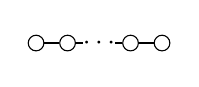
\begin{tikzpicture}[scale=0.4, baseline=-3pt, circ/.style={draw, circle, inner sep=2pt}]
        \node[circ] (1) at (0,0) {}; \node[circ] (2) at (1,0) {}; \node (3) at (2,0) {$\cdots$}; \node[circ] (4) at (3,0) {}; \node[circ] (5) at (4,0) {};
        \draw (1)--(2) (2)--(1.5,0) (2.5,0)--(4) (4)--(5);
    \end{tikzpicture} & $SL_{n+1}, PGL_{n+1}$ \\
    
    % --- Type B ---
    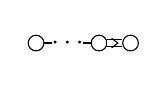
\begin{tikzpicture}[scale=0.4, baseline=-3pt, circ/.style={draw, circle, inner sep=2pt}]
        \node[circ] (1) at (0,0) {}; \node (2) at (1,0) {$\cdots$}; \node[circ] (3) at (2,0) {}; \node[circ] (4) at (3,0) {};
        \draw (1)--(0.5,0) (1.5,0)--(3);
        \draw[double, double distance=2pt] (3) -- (4);
        \draw (2.4,0.15) -- (2.6,0) -- (2.4,-0.15); % Arrow
    \end{tikzpicture} & $SO_{2n+1}$ \\

    % --- Type D ---
    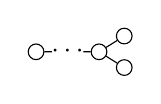
\begin{tikzpicture}[scale=0.4, baseline=-3pt, circ/.style={draw, circle, inner sep=2pt}]
        \node[circ] (1) at (0,0) {}; \node (2) at (1,0) {$\cdots$}; \node[circ] (3) at (2,0) {}; \node[circ] (4) at (2.8,0.5) {}; \node[circ] (5) at (2.8,-0.5) {};
        \draw (1)--(0.5,0) (1.5,0)--(3) (3)--(4) (3)--(5);
    \end{tikzpicture} & $SO_{2n}$ \\

    % --- Type E6 ---
    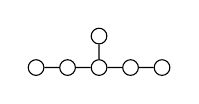
\begin{tikzpicture}[scale=0.4, baseline=-3pt, circ/.style={draw, circle, inner sep=2pt}]
        \node[circ] (1) at (0,0) {}; \node[circ] (2) at (1,0) {}; \node[circ] (3) at (2,0) {}; \node[circ] (4) at (3,0) {}; \node[circ] (5) at (4,0) {}; \node[circ] (6) at (2,1) {};
        \draw (1)--(2)--(3)--(4)--(5) (3)--(6);
    \end{tikzpicture} & $E_6$ \\

    % --- Type G2 ---
    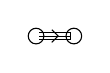
\begin{tikzpicture}[scale=0.4, baseline=-3pt, circ/.style={draw, circle, inner sep=2pt}]
        \node[circ] (1) at (0,0) {}; \node[circ] (2) at (1.2,0) {};
        \draw (1.1,0.1) -- (1.1,-0.1); % Triple line hack or use arrows
        \draw (1.1,0) -- (0.1,0); \draw (1.1,0.1) -- (0.1,0.1); \draw (1.1,-0.1) -- (0.1,-0.1);
        \draw (0.5,0.2) -- (0.7,0) -- (0.5,-0.2); % Arrowhead
    \end{tikzpicture} & $G_2$ \\
\end{tabular}
\fi


    \iffalse
    \begin{table}[h]
        \centering
        \begin{minipage}{0.40\textwidth}
            \centering
            % --- First table ---
            \begin{tabular}{|c|ccccc|}
                \hline
                & $[1^4]$ & $[211]$ & $[22]$ & $[31]$ & $[4]$ \\\hline
                $[F_4,1]$ & $0,\bar1$ & $0,\bar0$ & $0,\bar0$ & $0,\bar0$ & $0,\bar0$ \\\hline
                $[F_4(a_1),+]$ & $1,\bar1$ & $0,\bar1$ & $0,\bar0$ & $0,\bar0$ & $0,\bar0$ \\
                $[F_4(a_1),-]$ & $1,\bar1$ & $0,\bar0$ & $0,\bar0$ & $0,\bar0$ & $0,\bar0$ \\
                $[B_4,+]$ & $0,\bar0$ & $0,\bar1$ & $0,\bar0$ & $0,\bar0$ & $0,\bar0$ \\\hline
                $[F_4(a_2),+]$ & $1,\bar2$ & $1,\bar2$ & $0,\bar1$ & $0,\bar0$ & $0,\bar0$ \\
                $[F_4(a_2),-]$ & $0,\bar0$ & $0,\bar0$ & $0,\bar1$ & $0,\bar0$ & $0,\bar0$ \\
                $[C_3A_1,+]$ & $1,\bar2$ & $1,\bar2$ & $0,\bar0$ & $0,\bar0$ & $0,\bar0$ \\\hline
                $[B_4(711),+]$ & $0,\bar0$ & $0,\bar0$ & $0,\bar0$ & $0,\bar0$ & $0,\bar0$ \\
                $[B_4(711),-]$ & $0,\bar0$ & $0,\bar0$ & $0,\bar0$ & $0,\bar0$ & $0,\bar0$ \\\hline
                $[F_4(a_3),4]$ & $2,\bar{3}$ & $3,\bar{5}$ & $1,\bar1$ & $1,\bar2$ & $0,\bar0$ \\
                $[F_4(a_3),31]$ & $3,\bar2$ & $2,\bar2$ & $1,\bar0$ & $0,\bar0$ & $0,\bar0$ \\
                $[F_4(a_3),22]$ & $1,\bar0$ & $1,\bar1$ & $0,\bar0$ & $0,\bar1$ & $0,\bar0$ \\
                $[F_4(a_3),211]$ & $1,\bar0$ & $0,\bar0$ & $0,\bar0$ & $0,\bar0$ & $0,\bar0$ \\
                $[C_3(42)A_1,++]$ & $2,\bar{3}$ & $4,\bar{6}$ & $1,\bar1$ & $1,\bar2$ & $0,\bar0$ \\
                $[C_3(42)A_1,+-]$ & $2,\bar2$ & $1,\bar1$ & $1,\bar0$ & $0,\bar0$ & $0,\bar0$ \\
                $[B_4(531),1]$ & $0,\bar1$ & $2,\bar{4}$ & $0,\bar1$ & $1,\bar{3}$ & $0,\bar0$ \\
                $[B_4(531),\varepsilon'']$ & $0,\bar0$ & $1,\bar1$ & $0,\bar0$ & $0,\bar0$ & $0,\bar0$ \\
                $[B_4(531),\varepsilon']$ & $0,\bar0$ & $0,\bar0$ & $0,\bar0$ & $0,\bar1$ & $0,\bar0$ \\
                $[2A_2,1]$ & $1,\bar{3}$ & $2,\bar{4}$ & $1,\bar1$ & $1,\bar1$ & $0,\bar0$ \\
                $[A_1A_3,1]$ & $0,\bar1$ & $1,\bar{3}$ & $0,\bar1$ & $1,\bar2$ & $0,\bar0$ \\\hline
            \end{tabular}
            \caption{\centering{Parahoric restriction of \\ $F_4(F)$-representations labelled by the \\ distinguished unipotent $F_4(a_3)$ with respect to $K_2$}}
        \end{minipage}
        \hfill
        \begin{minipage}{0.40\textwidth}
            \centering
            \begin{tabular}{|c|ccccc|}
                \hline
                & $[1^4]$ & $[211]$ & $[22]$ & $[31]$ & $[4]$ \\\hline
                $\Pi(u,1,1)$ & $16,\bar{9}$ & $11,\bar{13}$ & $4,\bar1$ & $1,\bar{4}$ & $0,\bar0$ \\
                $\Pi(u,1,g_2)$ & $4,\bar{5}$ & $5,\bar{7}$ & $2,\bar1$ & $1,\bar2$ & $0,\bar0$ \\
                $\Pi(u,1,g_2')$ & $0,\bar1$ & $3,\bar{5}$ & $0,\bar1$ & $1,\bar{4}$ & $0,\bar0$ \\
                $\Pi(u,1,g_3)$ & $1,\bar{3}$ & $2,\bar{4}$ & $1,\bar1$ & $1,\bar1$ & $0,\bar0$ \\
                $\Pi(u,1,g_4)$ & $0,\bar1$ & $1,\bar{3}$ & $0,\bar1$ & $1,\bar2$ & $0,\bar0$ \\\hline
                $\Pi(u,g_2,1)$ & $4,\bar{5}$ & $5,\bar{7}$ & $2,\bar1$ & $1,\bar2$ & $0,\bar0$ \\
                $\Pi(u,g_2,g_2)$ & $4,\bar{5}$ & $5,\bar{7}$ & $2,\bar1$ & $1,\bar2$ & $0,\bar0$ \\
                $\Pi(u,g_2,\tau)$ & $0,\bar1$ & $3,\bar{5}$ & $0,\bar1$ & $1,\bar2$ & $0,\bar0$ \\
                $\Pi(u,g_2,g_2')$ & $0,\bar1$ & $3,\bar{5}$ & $0,\bar1$ & $1,\bar2$ & $0,\bar0$ \\\hline
                $\Pi(u,g_2',1)$ & $0,\bar1$ & $3,\bar{5}$ & $0,\bar1$ & $1,\bar{4}$ & $0,\bar0$ \\
                $\Pi(u,g_2',g_2)$ & $0,\bar1$ & $3,\bar{5}$ & $0,\bar1$ & $1,\bar2$ & $0,\bar0$ \\
                $\Pi(u,g_2',\gamma)$ & $0,\bar1$ & $1,\bar{3}$ & $0,\bar1$ & $1,\bar4$ & $0,\bar0$ \\
                $\Pi(u,g_2',g_2')$ & $0,\bar1$ & $3,\bar{5}$ & $0,\bar1$ & $1,\bar4$ & $0,\bar0$ \\
                $\Pi(u,g_2',g_4)$ & $0,\bar1$ & $1,\bar{3}$ & $0,\bar1$ & $1,\bar2$ & $0,\bar0$ \\\hline
                $\Pi(u,g_3,h)$ & $1,\bar{3}$ & $2,\bar{4}$ & $1,\bar1$ & $1,\bar1$ & $0,\bar0$ \\\hline
                $\Pi(u,g_4,h)$ & $0,\bar1$ & $1,\bar{3}$ & $0,\bar1$ & $1,\bar2$ & $0,\bar0$ \\\hline
            \end{tabular}
            \caption{\centering{Parahoric restrictions of the virtual characters $\Pi(u,s,h)$ where $u\in F_4(a_3)$ \\ with respect to $K_2$}}
        \end{minipage}
    \end{table}
    \newpage

    \begin{table}[!ht]
        \centering
        {\small
        \begin{tabular}{|c|cccc|cccc|cccc|}
            \hline
        & $[3,\cdot]$ & $[1,2]$ & $[11,1]$ & $[\cdot,1^3]$ & $[1,11]$ & $[1^3,\cdot]$ & $[\cdot,21]$ & $\theta_1$ & $[2,1]$ & $[21,\cdot]$ & $[\cdot,3]$ & $\theta_2$ \\\hline
        $\Pi(F_4(a_3),1,1)$ & $0,\bar0$ & $4,\bar{4}$ & $1,\bar2$ & $4,\bar2$ & $4,\bar{8}$ & $0,\bar1$ & $4,\bar{7}$ & $0,\bar0$ & $0,\bar{6}$ & $0,\bar0$ & $0,\bar{6}$ & $0,\bar0$\\
        $\Pi(F_4(a_3),1,g_2)$ & $0,\bar0$ & $2,\bar2$ & $1,\bar2$ & $2,\bar2$ & $2,\bar{4}$ & $0,\bar1$ & $2,\bar{3}$ & $0,\bar0$ & $0,\bar2$ & $0,\bar0$ & $0,\bar0$ & $0,\bar0$ \\
        $\Pi(F_4(a_3),1,g_2')$ & $0,\bar0$ & $0,\bar0$ & $1,\bar2$ & $4,\bar2$ & $4,\bar{4}$ & $0,\bar1$ & $0,-\bar1$ & $0,\bar0$ & $0,\bar2$ & $0,\bar0$ & $0,-\bar2$ & $0,\bar0$ \\
        $\Pi(F_4(a_3),1,g_3)$ & $0,\bar0$ & $1,\bar1$ & $1,\bar2$ & $1,\bar2$ & $1,\bar2$ & $0,\bar1$ & $1,\bar1$ & $0,\bar0$ & $0,\bar0$ & $0,\bar0$ & $0,\bar0$ & $0,\bar0$ \\
        $\Pi(F_4(a_3),1,g_4)$ & $0,\bar0$ & $0,\bar0$ & $1,\bar2$ & $2,\bar2$ & $2,\bar2$ & $0,\bar1$ & $0,-\bar1$ & $0,\bar0$ & $0,\bar0$ & $0,\bar0$ & $0,\bar0$ & $0,\bar0$ \\\hdashline
        $\Pi(F_4(a_3),g_2,1)$ & $0,\bar0$ & $2,\bar2$ & $1,\bar2$ & $2,\bar2$ & $2,\bar{4}$ & $0,\bar1$ & $2,\bar{3}$ & $0,\bar0$ & $0,\bar1$ & $0,\bar1$ & $0,\bar1$ & $0,\bar1$ \\
        $\Pi(F_4(a_3),g_2,g_2)$ & $0,\bar0$ & $2,\bar2$ & $1,\bar2$ & $2,\bar2$ & $2,\bar{4}$ & $0,\bar1$ & $2,\bar{3}$ & $0,\bar0$ & $0,\bar1$ & $0,\bar1$ & $0,\bar1$ & $0,-\bar1$ \\
        $\Pi(F_4(a_3),g_2,\tau)$ & $0,\bar0$ & $0,\bar0$ & $1,\bar2$ & $2,\bar2$ & $2,\bar2$ & $0,\bar1$ & $2,\bar1$ & $0,\bar0$ & $0,\bar1$ & $0,\bar1$ & $0,-\bar{1}$ & $0,\bar1$ \\
        $\Pi(F_4(a_3),g_2,g_2')$ & $0,\bar0$ & $0,\bar0$ & $1,\bar2$ & $2,\bar2$ & $2,\bar2$ & $0,\bar1$ & $2,\bar1$ & $0,\bar0$ & $0,\bar1$ & $0,\bar1$ & $0,-\bar{1}$ & $0,-\bar{1}$ \\\hdashline

        $\Pi(F_4(a_3),g_2',1)$ & $0,\bar0$ & $0,\bar0$ & $1,\bar2$ & $4,\bar2$ & $2,\bar2$ & $2,\bar{3}$ & $2,\bar1$ & $2,\bar2$ & $0,\bar0$ & $0,\bar2$ & $0,\bar0$ & $0,\bar2$\\

        $\Pi(F_4(a_3),g_2',g_2)$ & $0,\bar0$ & $0,\bar0$ & $1,\bar2$ & $2,\bar2$ & $2,\bar2$ & $0,\bar1$ & $2,\bar1$ & $0,\bar0$ & $0,\bar0$ & $0,\bar2$ & $0,\bar0$ & $0,\bar0$\\

        $\Pi(F_4(a_3),g_2',\gamma)$ & $0,\bar0$ & $0,\bar0$ & $1,\bar2$ & $4,\bar2$ & $2,\bar2$ & $2,\bar{3}$ & $0,-\bar{1}$ & $0,\bar0$ & $0,\bar0$ & $0,\bar0$ & $0,\bar0$ & $0,\bar0$\\

        $\Pi(F_4(a_3),g_2',g_2')$ & $0,\bar0$ & $0,\bar0$ & $1,\bar2$ & $4,\bar2$ & $2,\bar2$ & $2,\bar{3}$ & $2,\bar1$ & $-2,-\bar2$ & $0,\bar0$ & $0,\bar2$ & $0,\bar0$ & $0,-\bar2$\\

        $\Pi(F_4(a_3),g_2',g_4)$  & $0,\bar0$ & $0,\bar0$ & $1,\bar2$ & $2,\bar2$ & $2,\bar2$ & $0,\bar1$ & $0,-\bar1$ & $0,\bar0$ & $0,\bar0$ & $0,\bar0$ & $0,\bar0$ & $0,\bar0$ \\\hdashline

        $\Pi(F_4(a_3),g_3,h)$  & $0,\bar0$ & $1,\bar1$ & $1,\bar2$ & $1,\bar2$ & $1,\bar2$ & $0,\bar1$ & $1,\bar1$ & $0,\bar0$ & $0,\bar0$ & $0,\bar0$ & $0,\bar0$ & $0,\bar0$ \\\hdashline
        $\Pi(F_4(a_3),g_4,1/g_2')$ & {$0,\bar0$} & {$0,\bar0$} & {$1,\bar2$} & {$2,\bar2$} & {$1,\bar1$} & {$1,\bar2$} & {$1,\bar0$} & {$1,\bar1$} & {$0,\bar0$} & {$0,\bar0$} & {$0,\bar0$} & {$0,\bar0$} \\
        $\Pi(F_4(a_3),g_4,g_4^{\pm1})$ & {$0,\bar0$} & {$0,\bar0$} & {$1,\bar2$} & {$2,\bar2$} & {$1,\bar1$} & {$1,\bar2$} & {$1,\bar0$} & {$-1,-\bar1$} & {$0,\bar0$} & {$0,\bar0$} & {$0,\bar0$} & {$0,\bar0$} \\\hline
        \end{tabular}
        }
        \caption{Parahoric restrictions of the virtual characters $\Pi(u,s,h)$ with respect to $K_4$}
    \end{table}


    \fi
    .
    \newpage
    \begin{landscape}
    \subsection{Parahoric restriction tables for \texorpdfstring{$E_6$}{PDFstring}}
    \newpage
    
        \subsubsection{Iwahori-spherical \texorpdfstring{$E_6$}{PDFstring}-types}


        \begin{table}[ht]
        \centering
        \begin{adjustbox}{max width=\linewidth}
            \begin{tabular}{|c|c|c|c|}
                \hline
                & $J_0\longrightarrow E_6$ & $J_1\longrightarrow E_6$ & $J_6\longrightarrow E_6$ \\\hline

                $[E_6,1]$ & \multicolumn{3}{c|}{$\phi_{1,36}$} \\\hline

                $[E_6(a_1),1]$ & \multicolumn{3}{c|}{$\phi_{1,36}+\phi_{6,25}$} \\\hline

                $[E_6(a_3),+]$ & \multicolumn{3}{c|}{$\phi_{1,36}+\phi_{6,25}+\phi_{20,20}+\phi_{30,15}$} \\
                $[E_6(a_3),_]$ & \multicolumn{3}{c|}{$\phi_{6,25}+\phi_{15,17}$} \\
                $[A_1A_5,+]$ & \multicolumn{3}{c|}{$\phi_{1,36}+\phi_{15,16}+\phi_{20,20}$} \\
                $[A_1A_5,-]$ & \multicolumn{3}{c|}{$D_4[\epsilon]$} \\\hline

                $[D_4(71),1]$ & $\phi_{1,36}+\phi_{15,17}+\phi_{20,20}+\phi_{24,12}+\phi_{30,15}$ &  $\phi_{6,25}+\phi_{20,20}+\phi_{64,13}$ &  $\phi_{6,25}+\phi_{20,20}+\phi_{64,13}$ \\
                $[D_4(71),\theta]$ & $\phi_{6,25}+\phi_{20,20}+\phi_{64,13}$ & $\phi_{1,36}+\phi_{15,17}+\phi_{20,20}+\phi_{24,12}+\phi_{30,15}$ &  $\phi_{6,25}+\phi_{20,20}+\phi_{64,13}$  \\
                $[D_4(71),\theta^2]$ & $\phi_{6,25}+\phi_{20,20}+\phi_{64,13}$ &  $\phi_{6,25}+\phi_{20,20}+\phi_{64,13}$ & $\phi_{1,36}+\phi_{15,17}+\phi_{20,20}+\phi_{24,12}+\phi_{30,15}$ \\\hline
                

                $[D_4(a_1),1]$ & \multicolumn{3}{c|}{$\phi_{1,36}+\phi_{6,25}+\phi_{15,16}+3\phi_{20,20}+\phi_{24,12}+2\phi_{30,15}+\phi_{80,7}+2\phi_{60,11}+2\phi_{64,13}+\phi_{81,10}$}\\
                $[D_4(a_1),r]$ & \multicolumn{3}{c|}{$\phi_{6,25}+\phi_{15,17}+\phi_{20,20}+\phi_{30,15}+\phi_{90,8}+2\phi_{64,13}+\phi_{81,10}$}\\
                $[D_4(a_1),\epsilon]$ & \multicolumn{3}{c|}{$\phi_{20,10}+\phi_{15,17}$}\\\hline

                $[D_4(53),1]$ & $\phi_{1,36}+\phi_{6,25}+\phi_{20,10}+3\phi_{15,17}+\phi_{15,16}+2\phi_{20,20}+\phi_{24,12}+2\phi_{30,15}+\phi_{80,7}+2\phi_{64,13}+\phi_{81,10}$ & short & short\\
                $[D_4(53),\theta]$ & $\phi_{6,25}+\phi_{15,17}+2\phi_{20,20}+\phi_{30,15}+\phi_{90,8}+\phi_{60,11}+2\phi_{64,13}+\phi_{81,10}$ & long & short\\
                $[D_4(53),\theta^2]$ & $\phi_{6,25}+\phi_{15,17}+2\phi_{20,20}+\phi_{30,15}+\phi_{90,8}+\phi_{60,11}+2\phi_{64,13}+\phi_{81,10}$ & short  & long\\\hline

                $[3A_2,1\boxtimes1]$ & $\phi_{1,36}+\phi_{10,9}+2\phi_{15,16}+\phi_{24,12}+\phi_{30,15}$ & $\phi_{20,20}+\phi_{60,11}$ & $\phi_{20,20}+\phi_{60,11}$ \\
                $[3A_2,\theta\boxtimes1]$ & $E_6[\theta]$ & $0$ & $0$ \\
                $[3A_2,\theta^2\boxtimes1]$ & $E_6[\theta^2]$ & $0$ & $0$ \\
                $[3A_2,1\boxtimes\theta]$ & $\phi_{20,20}+\phi_{60,11}$ & $\phi_{1,36}+\phi_{10,9}+2\phi_{15,16}+\phi_{24,12}+\phi_{30,15}$ & $\phi_{20,20}+\phi_{60,11}$ \\
                $[3A_2,\theta\boxtimes\theta]$ & $0$ & $E_6[\theta]$ & $0$ \\
                $[3A_2,\theta^2\boxtimes\theta]$ & $0$ & $E_6[\theta^2]$ & $0$ \\
                $[3A_2,1\boxtimes\theta^2]$ & $\phi_{20,20}+\phi_{60,11}$ & $\phi_{20,20}+\phi_{60,11}$ & $\phi_{1,36}+\phi_{10,9}+2\phi_{15,16}+\phi_{24,12}+\phi_{30,15}$\\
                $[3A_2,\theta\boxtimes\theta^2]$ & $0$ & $0$ & $E_6[\theta]$ \\
                $[3A_2,\theta^2\boxtimes\theta^2]$ & $0$ & $0$ & $E_6[\theta^2]$ \\\hline

                $[D_4(3311),1]$ & \multicolumn{3}{c|}{$\phi_{1,36}+\phi_{10,9}+3\phi_{6,25}+\phi_{20,10}+3\phi_{15,17}+4\phi_{15,16}+8\phi_{20,20}+\phi_{24,6}+5\phi_{24,12}+\phi_{30,3}+8\phi_{30,15}+6\phi_{60,8}+9\phi_{80,7}+9\phi_{90,8}+3\phi_{60,5}+11\phi_{60,11}+2\phi_{64,4}+14\phi_{64,13}+6\phi_{81,6}+12\phi_{81,10}$} \\
                $[D_4(3311),\varepsilon]$ & \multicolumn{3}{c|}{$\phi_{6,25}+3\phi_{20,10}+\phi_{15,5}+3\phi_{15,17}+\phi_{15,16}+2\phi_{20,20}+\phi_{24,6}+\phi_{24,12}+3\phi_{30,15}+2\phi_{60,8}+3\phi_{80,7}+6\phi_{90,8}+\phi_{60,5}+3\phi_{60,11}+2\phi_{64,4}+6\phi_{64,13}+3\phi_{81,6}+6\phi_{81,10}$} \\\hline
            \end{tabular}
        \end{adjustbox}
        \caption{My Massive Triality Table}
        \label{tbl:E6_hyperspecialWJ0}
        \end{table}

        \iffalse

        \begin{table}
            \centering
            \caption{Parahoric restriction of $E_6(F)$-representations across $K_{J_0}$, $K_{J_1}$, $K_{J_6}$}
            \begin{tabular}{|c|c|c|c|}
            \hline
            & $J_0\longrightarrow E_6$ & $J_1\longrightarrow E_6$ & $J_6\longrightarrow E_6$ \\\hline

            $[E_6,1]$ & \multicolumn{3}{c}{$\phi_{1,36}$} \\\hline

            $[E_6(a_1),1]$ & \multicolumn{3}{c}{$\phi_{1,36}+\phi_{6,25}$} \\\hline

            $[E_6(a_3),+]$ & \multicolumn{3}{c}{$\phi_{1,36}+\phi_{6,25}+\phi_{20,20}+\phi_{30,15}$} \\
            $[E_6(a_3),_]$ & \multicolumn{3}{c}{$\phi_{6,25}+\phi_{15,17}$} \\
            $[A_1A_5,+]$ & \multicolumn{3}{c}{$\phi_{1,36}+\phi_{15,16}+\phi_{20,20}$} \\
            $[A_1A_5,-]$ & \multicolumn{3}{c}{$D_4[\epsilon]$} \\\hline

            $[D_4(71),1]$ & $\phi_{1,36}+\phi_{15,17}+\phi_{20,20}+\phi_{24,12}+\phi_{30,15}$ & short & short \\
            $[D_4(71),\theta]$ & $\phi_{6,25}+\phi_{20,20}+\phi_{64,13}$ & long & short  \\
            $[D_4(71),\theta^2]$ & $\phi_{6,25}+\phi_{20,20}+\phi_{64,13}$ & short & long \\\hline
            

            $[D_4(a_1),1]$ & \multicolumn{3}{c}{$\phi_{1,36}+\phi_{6,25}+\phi_{15,16}+3\phi_{20,20}+\phi_{24,12}+2\phi_{30,15}+\phi_{80,7}+2\phi_{60,11}+2\phi_{64,13}+\phi_{81,10}$}\\
            $[D_4(a_1),r]$ & \multicolumn{3}{c}{$\phi_{6,25}+\phi_{15,17}+\phi_{20,20}+\phi_{30,15}+\phi_{90,8}+2\phi_{64,13}+\phi_{81,10}$}\\
            $[D_4(a_1),\epsilon]$ & \multicolumn{3}{c}{$\phi_{20,10}+\phi_{15,17}$}\\\hline

            $[D_4(53),1]$ & $\phi_{1,36}+\phi_{6,25}+\phi_{20,10}+3\phi_{15,17}+\phi_{15,16}+2\phi_{20,20}+\phi_{24,12}+2\phi_{30,15}+\phi_{80,7}+2\phi_{64,13}+\phi_{81,10}$ & short & short\\
            $[D_4(53),\theta]$ & $\phi_{6,25}+\phi_{15,17}+2\phi_{20,20}+\phi_{30,15}+\phi_{90,8}+\phi_{60,11}+2\phi_{64,13}+\phi_{81,10}$ & long & short\\
            $[D_4(53),\theta^2]$ & $\phi_{6,25}+\phi_{15,17}+2\phi_{20,20}+\phi_{30,15}+\phi_{90,8}+\phi_{60,11}+2\phi_{64,13}+\phi_{81,10}$ & short  & long\\\hline

            $[3A_2,1\boxtimes1]$ & $\phi_{1,36}+\phi_{10,9}+2\phi_{15,16}+\phi_{24,12}+\phi_{30,15}$ & short & short \\
            $[3A_2,\theta\boxtimes1]$ & $E_6[\theta]$ & $0$ & $0$ \\
            $[3A_2,\theta^2\boxtimes1]$ & $E_6[\theta^2]$ & $0$ & $0$ \\
            $[3A_2,1\boxtimes\theta]$ & $\phi_{20,20}+\phi_{60,11}$ & long & short \\
            $[3A_2,\theta\boxtimes\theta]$ & $0$ & $E_6[\theta]$ & $0$ \\
            $[3A_2,\theta^2\boxtimes\theta]$ & $0$ & $E_6[\theta^2]$ & $0$ \\
            $[3A_2,1\boxtimes\theta^2]$ & $\phi_{20,20}+\phi_{60,11}$ & short & long\\
            $[3A_2,\theta\boxtimes\theta^2]$ & $0$ & $0$ & $E_6[\theta]$ \\
            $[3A_2,\theta^2\boxtimes\theta^2]$ & $0$ & $0$ & $E_6[\theta^2]$ \\\hline

            $[D_4(3311),1]$ & \multicolumn{3}{c}{$\phi_{1,36}+\phi_{10,9}+3\phi_{6,25}+\phi_{20,10}+3\phi_{15,17}+4\phi_{15,16}+8\phi_{20,20}+\phi_{24,6}+5\phi_{24,12}+\phi_{30,3}+8\phi_{30,15}+6\phi_{60,8}+9\phi_{80,7}+9\phi_{90,8}+3\phi_{60,5}+11\phi_{60,11}+2\phi_{64,4}+14\phi_{64,13}+6\phi_{81,6}+12\phi_{81,10}$} \\
            $[D_4(3311),\varepsilon]$ & \multicolumn{3}{c}{$\phi_{6,25}+3\phi_{20,10}+\phi{15,5}+3\phi_{15,17}+\phi_{15,16}+2\phi_{20,20}+\phi_{24,6}+\phi_{24,12}+3\phi_{30,15}+2\phi_{60,8}+3\phi_{80,7}+6\phi_{90,8}+\phi_{60,5}+3\phi_{60,11}+2\phi_{64,4}+6\phi_{64,13}+3\phi_{81,6}+6\phi_{81,10}$} \\\hline
            \end{tabular}
        \end{table}\fi
        \newpage
        \begin{table}
            \centering
            \begin{tabular}{|c|cccccccc|cccc|cccc|c|}
            \hline
                & $\phi_{80,7}$ & $\phi_{90,8}$ & $\phi_{20,10}$ & $\phi_{60,8}$ & $D_4[r]$ & $\phi_{10,9}$ & $E_6[\theta]$ & $E_6[\theta^2]$ & $\phi_{30,15}$ & $\phi_{15,17}$ & $\phi_{15,16}$ & $D_4[\epsilon]$ & $\phi_{30,3}$ & $\phi_{15,5}$ & $\phi_{15,4}$ & $D_4[1]$ & Fourier-stable \\\hline
                $\Pi(E_6,1,1)$  & 0 & 0 & 0 & 0 & 0 & 0 & 0 & 0 & 0 & 0 & 0 & 0 & 0 & 0 & 0 & 0 & $\phi_{1,36}$ \\\hline
                $\Pi(E_6(a_1),1,1)$  & 0 & 0 & 0 & 0 & 0 & 0 & 0 & 0 & 0 & 0 & 0 & 0 & 0 & 0 & 0 & 0 & $\phi_{1,36}+\phi_{6,25}$ \\\hline
                $\Pi(E_6(a_3),1,1)$  & 0 & 0 & 0 & 0 & 0 & 0 & 0 & 0 & 1 & 1 & 0 & 0 & 0 & 0 & 0 & 0 & $\Phi_{E_6(a_3)}$ \\
                $\Pi(E_6(a_3),1,g_2)$  & 0 & 0 & 0 & 0 & 0 & 0 & 0 & 0 & 1 & -1 & 0 & 0 & 0 & 0 & 0 & 0 & $\phi_{1,36}+\phi_{20,20}$ \\
                $\Pi(E_6(a_3),g_2,1)$ & 0 & 0 & 0 & 0 & 0 & 0 & 0 & 0 & 0 & 0 & 1 & 1 & 0 & 0 & 0 & 0 & $\phi_{1,36}+\phi_{20,20}$ \\
                $\Pi(E_6(a_3),g_2,g_2)$  & 0 & 0 & 0 & 0 & 0 & 0 & 0 & 0 & 0 & 0 & 1 & -1 & 0 & 0 & 0 & 0 & $\phi_{1,36}+\phi_{20,20}$ \\\hline
                $\Pi(D_4,s_3,w_3)$ & 0 & 0 & 0 & 0 & 0 & 0 & 0 & 0 & 1 & 1 & 0 & 0 & 0 & 0 & 0 & 0 & $\Phi_{D_4}$ \\
                $\Pi(D_4,s_3,w_3^2)$ & 0 & 0 & 0 & 0 & 0 & 0 & 0 & 0 & 1 & 1 & 0 & 0 & 0 & 0 & 0 & 0 & $\Phi_{D_4}$ \\\hline

                $\Pi(D_4(a_1),1,g_3)$ & 1 & -1 & 1 & 0 & 0 & 0 & 0 & 0 & 1 & 1 & 0 & 0 & 0 & 0 & 0 & 0 & $\Phi_{D_4(a_1)}^1$ \\
                $\Pi(D_4(a_1),z,g_3)$ & 1 & -1 & 1 & 0 & 0 & 0 & 0 & 0 & 1 & 1 & 0 & 0 & 0 & 0 & 0 & 0 & $\Phi_{D_4(a_1)}^2$ \\
                $\Pi(D_4(a_1),z^2,g_3)$ & 1 & -1 & 1 & 0 & 0 & 0 & 0 & 0 & 1 & 1 & 0 & 0 & 0 & 0 & 0 & 0 & $\Phi_{D_4(a_1)}^3$ \\
                $\Pi(D_4(a_1),g_3,1)$ & 0 & 0 & 0 & 0 & 0 & 1 & 1 & 1 & 1 & 1 & 0 & 0 & 0 & 0 & 0 & 0 & $\Phi_{D_4(a_1)}^1$ \\
                $\Pi(D_4(a_1),g_3,z)$ & 0 & 0 & 0 & 0 & 0 & 1 & 1 & 1 & 1 & 1 & 0 & 0 & 0 & 0 & 0 & 0 & $\Phi_{D_4(a_1)}^2$ \\
                $\Pi(D_4(a_1),g_3,z^2)$ & 0 & 0 & 0 & 0 & 0 & 1 & 1 & 1 & 1 & 1 & 0 & 0 & 0 & 0 & 0 & 0 & $\Phi_{D_4(a_1)}^3$ \\\hline

                $\Pi(A_2,s_{3,3}, w_{3,3})$ & 12 & 15 & 4 & 8 & 0 & 1 & 0 & 0 & 11 & 6 & 5 & 0 & 1 & 1 & 0 & 0 & $\Phi_{A_2}$ \\\hline            
            \end{tabular}
        \end{table}

        Where, in the above table, all $\Phi_{-}$ are Fourier-stable combinations of the irreducible characters of $E_6(F)$ that are easily calculated from Table \ref{tbl:E6_hyperspecialWJ0}.

        \newpage
        \subsubsection{Iwahori-spherical \texorpdfstring{$A_1\times A_5$}{PDFstring}-types}
        \begin{table}[ht]
            \centering
            \label{tab:e6_a1a5_restriction_final}
            \begin{tabular}{|c|ccccccccccc|}
            \hline
            $V$ & $[1^6]$ & $[21^4]$ & $[2^21^2]$ & $[222]$ & $[31^3]$ & $[321]$ & $[333]$ & $[41^2]$ & $[42]$ & $[51]$ & $[6]$ \\ \hline
            $[E_6, 1]$             & $0, \bar{1}$ & $0, \bar{0}$ & $0, \bar{0}$ & $0, \bar{0}$ & $0, \bar{0}$ & $0, \bar{0}$ & $0, \bar{0}$ & $0, \bar{0}$ & $0, \bar{0}$ & $0, \bar{0}$ & $0, \bar{0}$ \\ \hline

            $[E_6(a_1), 1]$        & $1, \bar{1}$ & $0, \bar{1}$ & $0, \bar{0}$ & $0, \bar{0}$ & $0, \bar{0}$ & $0, \bar{0}$ & $0, \bar{0}$ & $0, \bar{0}$ & $0, \bar{0}$ & $0, \bar{0}$ & $0, \bar{0}$ \\ \hline

            $[E_6(a_3), +]$        & $2, \bar{2}$ & $1, \bar{3}$ & $1, \bar{1}$ & $0, \bar{1}$ & $0, \bar{1}$ & $0, \bar{0}$ & $0, \bar{0}$ & $0, \bar{0}$ & $0, \bar{0}$ & $0, \bar{0}$ & $0, \bar{0}$ \\
            $[E_6(a_3), -]$        & $1, \bar{0}$ & $1, \bar{1}$ & $0, \bar{0}$ & $0, \bar{0}$ & $0, \bar{1}$ & $0, \bar{0}$ & $0, \bar{0}$ & $0, \bar{0}$ & $0, \bar{0}$ & $0, \bar{0}$ & $0, \bar{0}$ \\
            $[A_1A_5, +]$          & $1, \bar{2}$ & $0, \bar{2}$ & $1, \bar{1}$ & $0, \bar{1}$ & $0, \bar{0}$ & $0, \bar{0}$ & $0, \bar{0}$ & $0, \bar{0}$ & $0, \bar{0}$ & $0, \bar{0}$ & $0, \bar{0}$ \\ \hline

            $[D_4(71), 1]$         & $1, \bar{2}$ & $2, \bar{2}$ & $1, \bar{2}$ & $0, \bar{1}$ & $1, \bar{2}$ & $0, \bar{0}$ & $0, \bar{1}$ & $0, \bar{0}$ & $0, \bar{0}$ & $0, \bar{0}$ & $0, \bar{0}$ \\
            $[D_4(71), \theta]$    & $1, \bar{1}$ & $2, \bar{3}$ & $1, \bar{2}$ & $0, \bar{0}$ & $1, \bar{1}$ & $0, \bar{1}$ & $0, \bar{0}$ & $0, \bar{0}$ & $0, \bar{0}$ & $0, \bar{0}$ & $0, \bar{0}$ \\
            $[D_4(71), \theta^2]$  & $1, \bar{1}$ & $2, \bar{3}$ & $1, \bar{2}$ & $0, \bar{0}$ & $1, \bar{1}$ & $0, \bar{1}$ & $0, \bar{0}$ & $0, \bar{0}$ & $0, \bar{0}$ & $0, \bar{0}$ & $0, \bar{0}$ \\ \hline
            
            $[D_4(a_1), 1]$        & $3, \bar{5}$ & $6, \bar{10}$ & $7, \bar{10}$ & $2, \bar{5}$ & $4, \bar{6}$ & $4, \bar{6}$ & $1, \bar{1}$ & $1, \bar{1}$ & $0, \bar{1}$ & $0, \bar{0}$ & $0, \bar{0}$ \\ 
            $[D_4(a_1), \epsilon]$  & $0, \bar{0}$ & $1, \bar{0}$ & $0, \bar{0}$ & $0, \bar{0}$ & $1, \bar{1}$ & $0, \bar{0}$ & $0, \bar{0}$ & $0, \bar{1}$ & $0, \bar{0}$ & $0, \bar{0}$ & $0, \bar{0}$ \\ 
            $[D_4(a_1), r]$        & $2, \bar{1}$ & $5, \bar{5}$ & $4, \bar{4}$ & $1, \bar{1}$ & $4, \bar{6}$ & $2, \bar{4}$ & $0, \bar{0}$ & $1, \bar{2}$ & $0, \bar{1}$ & $0, \bar{0}$ & $0, \bar{0}$ \\ 
            $[D_4(53), 1]$         & $3, \bar{3}$ & $5, \bar{6}$ & $5, \bar{6}$ & $2, \bar{3}$ & $5, \bar{7}$ & $2, \bar{4}$ & $1, \bar{1}$ & $1, \bar{2}$ & $0, \bar{1}$ & $0, \bar{0}$ & $0, \bar{0}$ \\ 
            $[D_4(53), \theta]$    & $2, \bar{2}$ & $6, \bar{7}$ & $5, \bar{6}$ & $1, \bar{2}$ & $4, \bar{6}$ & $3, \bar{5}$ & $0, \bar{0}$ & $1, \bar{2}$ & $0, \bar{1}$ & $0, \bar{0}$ & $0, \bar{0}$ \\ 
            $[D_4(53), \theta^2]$  & $2, \bar{2}$ & $6, \bar{7}$ & $5, \bar{6}$ & $1, \bar{2}$ & $4, \bar{6}$ & $3, \bar{5}$ & $0, \bar{0}$ & $1, \bar{2}$ & $0, \bar{1}$ & $0, \bar{0}$ & $0, \bar{0}$ \\ 
            $[3A_2, 1\boxtimes1]$            & $1, \bar{2}$ & $0, \bar{1}$ & $1, \bar{2}$ & $1, \bar{2}$ & $1, \bar{1}$ & $0, \bar{0}$ & $1, \bar{1}$ & $0, \bar{0}$ & $0, \bar{0}$ & $0, \bar{0}$ & $0, \bar{0}$ \\ 
            $[3A_2, 1\boxtimes\theta]$       & $0, \bar{1}$ & $1, \bar{2}$ & $1, \bar{2}$ & $0, \bar{1}$ & $0, \bar{0}$ & $1, \bar{1}$ & $0, \bar{0}$ & $0, \bar{0}$ & $0, \bar{0}$ & $0, \bar{0}$ & $0, \bar{0}$ \\ 
            $[3A_2, 1\boxtimes\theta^2]$     & $0, \bar{1}$ & $1, \bar{2}$ & $1, \bar{2}$ & $0, \bar{1}$ & $0, \bar{0}$ & $1, \bar{1}$ & $0, \bar{0}$ & $0, \bar{0}$ & $0, \bar{0}$ & $0, \bar{0}$ & $0, \bar{0}$ \\ \hline

            $[D_4(3311), 1]$       & $1, \bar{0}$ & $8, \bar{6}$ & $24, \bar{18}$ & $17, \bar{14}$ & $31, \bar{27}$ & $70, \bar{58}$ & $29, \bar{23}$ & $55, \bar{47}$ & $60, \bar{51}$ & $44, \bar{37}$ & $13, \bar{11}$ \\ 
            $[D_4(3311), \epsilon]$ & $0, \bar{0}$ & $6, \bar{3}$ & $12, \bar{9}$ & $6, \bar{4}$ & $21, \bar{15}$ & $30, \bar{26}$ & $9, \bar{10}$ & $27, \bar{25}$ & $21, \bar{21}$ & $15, \bar{17}$ & $3, \bar{4}$ \\ \hline
            \end{tabular}
            \caption{Parahoric restriction of $E_6(F)$-Iwahori spherical representations with respect to $K_{J_2}$}
        \end{table}

        
        \begin{table}[ht]
            \centering
            \label{tab:pi_combinations}
            \begin{tabular}{|c|ccccccccccc|}
            \hline
            Row Label & $[1^6]$ & $[21^4]$ & $[2^21^2]$ & $[222]$ & $[31^3]$ & $[321]$ & $[333]$ & $[41^2]$ & $[42]$ & $[51]$ & $[6]$ \\ \hline
            $\Pi(E_6,1,1)$          & $0, \bar{1}$ & $0, \bar{0}$ & $0, \bar{0}$ & $0, \bar{0}$ & $0, \bar{0}$ & $0, \bar{0}$ & $0, \bar{0}$ & $0, \bar{0}$ & $0, \bar{0}$ & $0, \bar{0}$ & $0, \bar{0}$ \\ \hline
            $\Pi(E_6(a_1),1,1)$     & $1, \bar{1}$ & $0, \bar{1}$ & $0, \bar{0}$ & $0, \bar{0}$ & $0, \bar{0}$ & $0, \bar{0}$ & $0, \bar{0}$ & $0, \bar{0}$ & $0, \bar{0}$ & $0, \bar{0}$ & $0, \bar{0}$ \\ \hline
            $\Pi(E_6(a_3),1,1)$     & $3, \bar{2}$ & $2, \bar{4}$ & $1, \bar{1}$ & $0, \bar{1}$ & $0, \bar{2}$ & $0, \bar{0}$ & $0, \bar{0}$ & $0, \bar{0}$ & $0, \bar{0}$ & $0, \bar{0}$ & $0, \bar{0}$ \\ 
            $\Pi(E_6(a_3),1,g_2)$   & $1, \bar{2}$ & $0, \bar{2}$ & $1, \bar{1}$ & $0, \bar{1}$ & $0, \bar{0}$ & $0, \bar{0}$ & $0, \bar{0}$ & $0, \bar{0}$ & $0, \bar{0}$ & $0, \bar{0}$ & $0, \bar{0}$ \\ 
            $\Pi(E_6(a_3),g_2,1)$   & $1, \bar{2}$ & $0, \bar{2}$ & $1, \bar{1}$ & $0, \bar{1}$ & $0, \bar{0}$ & $0, \bar{0}$ & $0, \bar{0}$ & $0, \bar{0}$ & $0, \bar{0}$ & $0, \bar{0}$ & $0, \bar{0}$ \\
            $\Pi(E_6(a_3),g_2,g_2)$ & $1, \bar{2}$ & $0, \bar{2}$ & $1, \bar{1}$ & $0, \bar{1}$ & $0, \bar{0}$ & $0, \bar{0}$ & $0, \bar{0}$ & $0, \bar{0}$ & $0, \bar{0}$ & $0, \bar{0}$ & $0, \bar{0}$ \\ \hline
            $\Pi(D_4,s_3,w_3)$      & $0, \bar{1}$ & $0, -\bar{1}$ & $0, \bar{0}$ & $0, \bar{1}$ & $0, \bar{1}$ & $0, -\bar{1}$ & $0, \bar{1}$ & $0, \bar{0}$ & $0, \bar{0}$ & $0, \bar{0}$ & $0, \bar{0}$ \\ 
            $\Pi(D_4,s_3,w_3^{-1})$ & $0, \bar{1}$ & $0, -\bar{1}$ & $0, \bar{0}$ & $0, \bar{1}$ & $0, \bar{1}$ & $0, -\bar{1}$ & $0, \bar{1}$ & $0, \bar{0}$ & $0, \bar{0}$ & $0, \bar{0}$ & $0, \bar{0}$ \\ \hline
            $\Pi(D_4(a_1),1,g_3)$   & $1, \bar{4}$ & $2, \bar{5}$ & $3, \bar{6}$ & $1, \bar{4}$ & $1, \bar{1}$ & $2, \bar{2}$ & $1, \bar{1}$ & $0, \bar{0}$ & $0, \bar{0}$ & $0, \bar{0}$ & $0, \bar{0}$ \\ 
            $\Pi(D_4(a_1),z,g_3)$   & $1, \bar{1}$ & $-1, -\bar{1}$ & $0, \bar{0}$ & $1, \bar{1}$ & $1, \bar{1}$ & $-1, -\bar{1}$ & $1, \bar{1}$ & $0, \bar{0}$ & $0, \bar{0}$ & $0, \bar{0}$ & $0, \bar{0}$ \\ 
            $\Pi(D_4(a_1),z,g_3^{-1})$ & $1, \bar{1}$ & $-1, -\bar{1}$ & $0, \bar{0}$ & $1, \bar{1}$ & $1, \bar{1}$ & $-1, -\bar{1}$ & $1, \bar{1}$ & $0, \bar{0}$ & $0, \bar{0}$ & $0, \bar{0}$ & $0, \bar{0}$ \\ 
            $\Pi(D_4(a_1),g_3,1)$   & $1, \bar{4}$ & $2, \bar{5}$ & $3, \bar{6}$ & $1, \bar{4}$ & $1, \bar{1}$ & $2, \bar{2}$ & $1, \bar{1}$ & $0, \bar{0}$ & $0, \bar{0}$ & $0, \bar{0}$ & $0, \bar{0}$ \\ 
            $\Pi(D_4(a_1),g_3,z)$   & $1, \bar{1}$ & $-1, -\bar{1}$ & $0, \bar{0}$ & $1, \bar{1}$ & $1, \bar{1}$ & $-1, -\bar{1}$ & $1, \bar{1}$ & $0, \bar{0}$ & $0, \bar{0}$ & $0, \bar{0}$ & $0, \bar{0}$ \\ 
            $\Pi(D_4(a_1),g_3,z^2)$ & $1, \bar{1}$ & $-1, -\bar{1}$ & $0, \bar{0}$ & $1, \bar{1}$ & $1, \bar{1}$ & $-1, -\bar{1}$ & $1, \bar{1}$ & $0, \bar{0}$ & $0, \bar{0}$ & $0, \bar{0}$ & $0, \bar{0}$ \\ \hline
            $\Pi(A_2,s_{3,3},w_{3,3})$ & $1, \bar{0}$ & $14, \bar{9}$ & $36, \bar{27}$ & $23, \bar{18}$ & $52, \bar{42}$ & $100, \bar{84}$ & $38, \bar{33}$ & $82, \bar{72}$ & $81, \bar{72}$ & $59, \bar{54}$ & $16, \bar{15}$ \\ \hline
            
            \end{tabular}
            \caption{Parahoric restriction of $\Pi(u,s,h)$ with respect to $K_{J_2}$}
        \end{table}
        
        \begin{table}[ht]
            \centering
            \label{tab:e6_WJ3_restriction_final}
            \begin{tabular}{|c|ccccccccccc|}
            \hline
            $V$ & $[1^6]$ & $[21^4]$ & $[2^21^2]$ & $[222]$ & $[31^3]$ & $[321]$ & $[333]$ & $[41^2]$ & $[42]$ & $[51]$ & $[6]$ \\ \hline
            $[E_6, 1]$             & $0, \bar{1}$ & $0, \bar{0}$ & $0, \bar{0}$ & $0, \bar{0}$ & $0, \bar{0}$ & $0, \bar{0}$ & $0, \bar{0}$ & $0, \bar{0}$ & $0, \bar{0}$ & $0, \bar{0}$ & $0, \bar{0}$ \\ \hline

            $[E_6(a_1), 1]$        & $1, \bar{1}$ & $0, \bar{1}$ & $0, \bar{0}$ & $0, \bar{0}$ & $0, \bar{0}$ & $0, \bar{0}$ & $0, \bar{0}$ & $0, \bar{0}$ & $0, \bar{0}$ & $0, \bar{0}$ & $0, \bar{0}$ \\ \hline

            $[E_6(a_3), +]$        & $2, \bar{2}$ & $1, \bar{3}$ & $1, \bar{1}$ & $0, \bar{1}$ & $0, \bar{1}$ & $0, \bar{0}$ & $0, \bar{0}$ & $0, \bar{0}$ & $0, \bar{0}$ & $0, \bar{0}$ & $0, \bar{0}$ \\
            $[E_6(a_3), -]$        & $1, \bar{0}$ & $1, \bar{1}$ & $0, \bar{0}$ & $0, \bar{0}$ & $0, \bar{1}$ & $0, \bar{0}$ & $0, \bar{0}$ & $0, \bar{0}$ & $0, \bar{0}$ & $0, \bar{0}$ & $0, \bar{0}$ \\
            $[A_1A_5, +]$          & $1, \bar{2}$ & $0, \bar{2}$ & $1, \bar{1}$ & $0, \bar{1}$ & $0, \bar{0}$ & $0, \bar{0}$ & $0, \bar{0}$ & $0, \bar{0}$ & $0, \bar{0}$ & $0, \bar{0}$ & $0, \bar{0}$ \\ \hline

            $[D_4(71), 1]$         & $1, \bar{1}$ & $2, \bar{3}$ & $1, \bar{2}$ & $0, \bar{0}$ & $1, \bar{1}$ & $0, \bar{1}$ & $0, \bar{0}$ & $0, \bar{0}$ & $0, \bar{0}$ & $0, \bar{0}$ & $0, \bar{0}$ \\ 
            $[D_4(71), \theta]$    & $1, \bar{1}$ & $2, \bar{3}$ & $1, \bar{2}$ & $0, \bar{0}$ & $1, \bar{1}$ & $0, \bar{1}$ & $0, \bar{0}$ & $0, \bar{0}$ & $0, \bar{0}$ & $0, \bar{0}$ & $0, \bar{0}$ \\
            $[D_4(71), \theta^2]$  & $1, \bar{2}$ & $2, \bar{2}$ & $1, \bar{2}$ & $0, \bar{1}$ & $1, \bar{2}$ & $0, \bar{0}$ & $0, \bar{1}$ & $0, \bar{0}$ & $0, \bar{0}$ & $0, \bar{0}$ & $0, \bar{0}$ \\\hline
            
            $[D_4(a_1), 1]$        & $3, \bar{5}$ & $6, \bar{10}$ & $7, \bar{10}$ & $2, \bar{5}$ & $4, \bar{6}$ & $4, \bar{6}$ & $1, \bar{1}$ & $1, \bar{1}$ & $0, \bar{1}$ & $0, \bar{0}$ & $0, \bar{0}$ \\ 
            $[D_4(a_1), \epsilon]$  & $0, \bar{0}$ & $1, \bar{0}$ & $0, \bar{0}$ & $0, \bar{0}$ & $1, \bar{1}$ & $0, \bar{0}$ & $0, \bar{0}$ & $0, \bar{1}$ & $0, \bar{0}$ & $0, \bar{0}$ & $0, \bar{0}$ \\ 
            $[D_4(a_1), r]$        & $2, \bar{1}$ & $5, \bar{5}$ & $4, \bar{4}$ & $1, \bar{1}$ & $4, \bar{6}$ & $2, \bar{4}$ & $0, \bar{0}$ & $1, \bar{2}$ & $0, \bar{1}$ & $0, \bar{0}$ & $0, \bar{0}$ \\ 
            $[D_4(53), 1]$         & $2, \bar{2}$ & $6, \bar{7}$ & $5, \bar{6}$ & $1, \bar{2}$ & $4, \bar{6}$ & $3, \bar{5}$ & $0, \bar{0}$ & $1, \bar{2}$ & $0, \bar{1}$ & $0, \bar{0}$ & $0, \bar{0}$ \\
            $[D_4(53), \theta]$    & $2, \bar{2}$ & $6, \bar{7}$ & $5, \bar{6}$ & $1, \bar{2}$ & $4, \bar{6}$ & $3, \bar{5}$ & $0, \bar{0}$ & $1, \bar{2}$ & $0, \bar{1}$ & $0, \bar{0}$ & $0, \bar{0}$ \\ 
            $[D_4(53), \theta^2]$  & $3, \bar{3}$ & $5, \bar{6}$ & $5, \bar{6}$ & $2, \bar{3}$ & $5, \bar{7}$ & $2, \bar{4}$ & $1, \bar{1}$ & $1, \bar{2}$ & $0, \bar{1}$ & $0, \bar{0}$ & $0, \bar{0}$ \\ 
            $[3A_2, 1\boxtimes1]$            & $0, \bar{1}$ & $1, \bar{2}$ & $1, \bar{2}$ & $0, \bar{1}$ & $0, \bar{0}$ & $1, \bar{1}$ & $0, \bar{0}$ & $0, \bar{0}$ & $0, \bar{0}$ & $0, \bar{0}$ & $0, \bar{0}$ \\
            $[3A_2, 1\boxtimes\theta]$       & $1, \bar{2}$ & $0, \bar{1}$ & $1, \bar{2}$ & $1, \bar{2}$ & $1, \bar{1}$ & $0, \bar{0}$ & $1, \bar{1}$ & $0, \bar{0}$ & $0, \bar{0}$ & $0, \bar{0}$ & $0, \bar{0}$ \\ 
            $[3A_2, 1\boxtimes\theta^2]$     & $0, \bar{1}$ & $1, \bar{2}$ & $1, \bar{2}$ & $0, \bar{1}$ & $0, \bar{0}$ & $1, \bar{1}$ & $0, \bar{0}$ & $0, \bar{0}$ & $0, \bar{0}$ & $0, \bar{0}$ & $0, \bar{0}$ \\ \hline

            $[D_4(3311), 1]$       & $1, \bar{0}$ & $8, \bar{6}$ & $24, \bar{18}$ & $17, \bar{14}$ & $31, \bar{27}$ & $70, \bar{58}$ & $29, \bar{23}$ & $55, \bar{47}$ & $60, \bar{51}$ & $44, \bar{37}$ & $13, \bar{11}$ \\ 
            $[D_4(3311), \epsilon]$ & $0, \bar{0}$ & $6, \bar{3}$ & $12, \bar{9}$ & $6, \bar{4}$ & $21, \bar{15}$ & $30, \bar{26}$ & $9, \bar{10}$ & $27, \bar{25}$ & $21, \bar{21}$ & $15, \bar{17}$ & $3, \bar{4}$ \\ \hline
            \end{tabular}
            \caption{Parahoric restriction of $E_6(F)$-Iwahori spherical representations with respect to $K_{J_3}$}
        \end{table}


        \begin{table}[ht]
            \centering
            \label{tab:e6_WJ3_restriction_final}
            \begin{tabular}{|c|ccccccccccc|}
            \hline
            $V$ & $[1^6]$ & $[21^4]$ & $[2^21^2]$ & $[222]$ & $[31^3]$ & $[321]$ & $[333]$ & $[41^2]$ & $[42]$ & $[51]$ & $[6]$ \\ \hline
            $[E_6, 1]$             & $0, \bar{1}$ & $0, \bar{0}$ & $0, \bar{0}$ & $0, \bar{0}$ & $0, \bar{0}$ & $0, \bar{0}$ & $0, \bar{0}$ & $0, \bar{0}$ & $0, \bar{0}$ & $0, \bar{0}$ & $0, \bar{0}$ \\ \hline

            $[E_6(a_1), 1]$        & $1, \bar{1}$ & $0, \bar{1}$ & $0, \bar{0}$ & $0, \bar{0}$ & $0, \bar{0}$ & $0, \bar{0}$ & $0, \bar{0}$ & $0, \bar{0}$ & $0, \bar{0}$ & $0, \bar{0}$ & $0, \bar{0}$ \\ \hline

            $[E_6(a_3), +]$        & $2, \bar{2}$ & $1, \bar{3}$ & $1, \bar{1}$ & $0, \bar{1}$ & $0, \bar{1}$ & $0, \bar{0}$ & $0, \bar{0}$ & $0, \bar{0}$ & $0, \bar{0}$ & $0, \bar{0}$ & $0, \bar{0}$ \\
            $[E_6(a_3), -]$        & $1, \bar{0}$ & $1, \bar{1}$ & $0, \bar{0}$ & $0, \bar{0}$ & $0, \bar{1}$ & $0, \bar{0}$ & $0, \bar{0}$ & $0, \bar{0}$ & $0, \bar{0}$ & $0, \bar{0}$ & $0, \bar{0}$ \\
            $[A_1A_5, +]$          & $1, \bar{2}$ & $0, \bar{2}$ & $1, \bar{1}$ & $0, \bar{1}$ & $0, \bar{0}$ & $0, \bar{0}$ & $0, \bar{0}$ & $0, \bar{0}$ & $0, \bar{0}$ & $0, \bar{0}$ & $0, \bar{0}$ \\ \hline

            $[D_4(71), 1]$         & $1, \bar{1}$ & $2, \bar{3}$ & $1, \bar{2}$ & $0, \bar{0}$ & $1, \bar{1}$ & $0, \bar{1}$ & $0, \bar{0}$ & $0, \bar{0}$ & $0, \bar{0}$ & $0, \bar{0}$ & $0, \bar{0}$ \\ 
            $[D_4(71), \theta]$    & $1, \bar{2}$ & $2, \bar{2}$ & $1, \bar{2}$ & $0, \bar{1}$ & $1, \bar{2}$ & $0, \bar{0}$ & $0, \bar{1}$ & $0, \bar{0}$ & $0, \bar{0}$ & $0, \bar{0}$ & $0, \bar{0}$ \\
            $[D_4(71), \theta^2]$  & $1, \bar{1}$ & $2, \bar{3}$ & $1, \bar{2}$ & $0, \bar{0}$ & $1, \bar{1}$ & $0, \bar{1}$ & $0, \bar{0}$ & $0, \bar{0}$ & $0, \bar{0}$ & $0, \bar{0}$ & $0, \bar{0}$ \\\hline
            
            $[D_4(a_1), 1]$        & $3, \bar{5}$ & $6, \bar{10}$ & $7, \bar{10}$ & $2, \bar{5}$ & $4, \bar{6}$ & $4, \bar{6}$ & $1, \bar{1}$ & $1, \bar{1}$ & $0, \bar{1}$ & $0, \bar{0}$ & $0, \bar{0}$ \\ 
            $[D_4(a_1), \epsilon]$  & $0, \bar{0}$ & $1, \bar{0}$ & $0, \bar{0}$ & $0, \bar{0}$ & $1, \bar{1}$ & $0, \bar{0}$ & $0, \bar{0}$ & $0, \bar{1}$ & $0, \bar{0}$ & $0, \bar{0}$ & $0, \bar{0}$ \\ 
            $[D_4(a_1), r]$        & $2, \bar{1}$ & $5, \bar{5}$ & $4, \bar{4}$ & $1, \bar{1}$ & $4, \bar{6}$ & $2, \bar{4}$ & $0, \bar{0}$ & $1, \bar{2}$ & $0, \bar{1}$ & $0, \bar{0}$ & $0, \bar{0}$ \\ 
            $[D_4(53), 1]$         & $2, \bar{2}$ & $6, \bar{7}$ & $5, \bar{6}$ & $1, \bar{2}$ & $4, \bar{6}$ & $3, \bar{5}$ & $0, \bar{0}$ & $1, \bar{2}$ & $0, \bar{1}$ & $0, \bar{0}$ & $0, \bar{0}$ \\
            $[D_4(53), \theta]$    & $3, \bar{3}$ & $5, \bar{6}$ & $5, \bar{6}$ & $2, \bar{3}$ & $5, \bar{7}$ & $2, \bar{4}$ & $1, \bar{1}$ & $1, \bar{2}$ & $0, \bar{1}$ & $0, \bar{0}$ & $0, \bar{0}$ \\ 
            $[D_4(53), \theta^2]$  & $2, \bar{2}$ & $6, \bar{7}$ & $5, \bar{6}$ & $1, \bar{2}$ & $4, \bar{6}$ & $3, \bar{5}$ & $0, \bar{0}$ & $1, \bar{2}$ & $0, \bar{1}$ & $0, \bar{0}$ & $0, \bar{0}$ \\
            $[3A_2, 1\boxtimes1]$            & $0, \bar{1}$ & $1, \bar{2}$ & $1, \bar{2}$ & $0, \bar{1}$ & $0, \bar{0}$ & $1, \bar{1}$ & $0, \bar{0}$ & $0, \bar{0}$ & $0, \bar{0}$ & $0, \bar{0}$ & $0, \bar{0}$ \\
            $[3A_2, 1\boxtimes\theta]$       & $0, \bar{1}$ & $1, \bar{2}$ & $1, \bar{2}$ & $0, \bar{1}$ & $0, \bar{0}$ & $1, \bar{1}$ & $0, \bar{0}$ & $0, \bar{0}$ & $0, \bar{0}$ & $0, \bar{0}$ & $0, \bar{0}$ \\
            $[3A_2, 1\boxtimes\theta^2]$     & $1, \bar{2}$ & $0, \bar{1}$ & $1, \bar{2}$ & $1, \bar{2}$ & $1, \bar{1}$ & $0, \bar{0}$ & $1, \bar{1}$ & $0, \bar{0}$ & $0, \bar{0}$ & $0, \bar{0}$ & $0, \bar{0}$ \\ \hline

            $[D_4(3311), 1]$       & $1, \bar{0}$ & $8, \bar{6}$ & $24, \bar{18}$ & $17, \bar{14}$ & $31, \bar{27}$ & $70, \bar{58}$ & $29, \bar{23}$ & $55, \bar{47}$ & $60, \bar{51}$ & $44, \bar{37}$ & $13, \bar{11}$ \\ 
            $[D_4(3311), \epsilon]$ & $0, \bar{0}$ & $6, \bar{3}$ & $12, \bar{9}$ & $6, \bar{4}$ & $21, \bar{15}$ & $30, \bar{26}$ & $9, \bar{10}$ & $27, \bar{25}$ & $21, \bar{21}$ & $15, \bar{17}$ & $3, \bar{4}$ \\ \hline
            \end{tabular}
            \caption{Parahoric restriction of $E_6(F)$-Iwahori spherical representations with respect to $K_{J_5}$}
        \end{table}        



        
        
        
        \newpage
        
        
        
        \begin{table}[ht]
            \centering
            \caption{Parahoric restriction of $E_6(F)$-representations with respect to Iwahori-spherical $A_2A_2A_2$-types}
            \label{tab:e6_a2a2a2_restriction}
            \begin{tabular}{|c|cccccccccc|}
            \hline
            $V$ & $[\varepsilon\varepsilon\varepsilon]$ & $[\varepsilon\varepsilon r]$ & $[\varepsilon\varepsilon 1]$ & $[\varepsilon r r]$ & $[\varepsilon r 1]$ & $[\varepsilon 1 1]$ & $[r r r]$ & $[r r 1]$ & $[r 1 1]$ & $[1 1 1]$ \\ \hline
            $[E_6, 1]$             & 1 & 0 & 0 & 0 & 0 & 0 & 0 & 0 & 0 & 0 \\ \hline
            $[E_6(a_1), 1]$        & 1 & 1 & 0 & 0 & 0 & 0 & 0 & 0 & 0 & 0\\ \hline
            $[E_6(a_3), +]$        & 4 & 3 & 1 & 2 & 0 & 0 & 1 & 0 & 0 & 0\\ 
            $[E_6(a_3), -]$        & 0 & 1 & 1 & 1 & 0 & 0 & 0 & 0 & 0 & 0\\ 
            $[A_1A_5, +]$          & 4 & 2 & 0 & 1 & 0 & 0 & 1 & 0 & 0 & 0\\ \hline
            
            \iffalse
            $[D_4(71), 1]$         & 5 & 2 & 2 & 4 & 0 & 0 & 0 & 0 & 0 & 0\\ 
            $[D_4(71), \theta]$    & 2 & 4 & 0 & 3 & 1 & 0 & 2 & 0 & 0 & 0\\ 
            $[D_4(71), \theta^2]$  & 2 & 4 & 0 & 3 & 1 & 0 & 2 & 0 & 0 & 0\\ \hline
            \fi

            $[D_4(71), 1]$         & 3 & 3,4,3 & 1,0,1 & 3,4,3 & 1,0,1,0,1,1 & 0,1,0 & 2 & 0 & 0 & 0 \\ 
            $[D_4(71), \theta]$    & 3 & 4,3,3 & 0,1,1 & 3,3,4 & 0,1,0,1,1,1 & 0,0,1 & 2 & 0 & 0 & 0 \\
            $[D_4(71), \theta^2]$  & 3 & 3,3,4 & 1,1,0 & 4,3,3 & 1,1,1,1,0,0 & 1,0,0 & 2 & 0 & 0 & 0 \\ \hline

            $[D_4(a_1), 1]$        & 15 & 15 & 3 & 17 & 4 & 1 & 19 & 4 & 1 & 0 \\ 
            $[D_4(a_1), \epsilon]$  & 0 & 0 & 1 & 1 & 1 & 0 & 1 & 0 & 0 & 0\\ 
            $[D_4(a_1), r]$        & 3 & 8 & 4 & 11 & 4 & 1 & 11 & 3 & 0 & 0\\\hline

            \iffalse
            $[D_4(53), 1]$         & 7 & 11 & 4 & 12 & 5 & 1 & 16 & 2 & 1 & 0\\ 
            $[D_4(53), \theta]$    & 7 & 10 & 4 & 14 & 4 & 1 & 13 & 4 & 0 & 0\\ 
            $[D_4(53), \theta^2]$  & 7 & 10 & 4 & 14 & 4 & 1 & 13 & 4 & 0 & 0\\ \hline
            \fi

            $[D_4(53), 1]$         & 7 & 10,11,10 & 4 & 13,14,13 & 5,4,4,4,4,5 & 1 & 14 & 3,4,3 & 0,1,0 & 0 \\
            $[D_4(53), \theta]$    & 7 & 10,10,11 & 4 & 14,13,13 & 4,4,5,5,4,4 & 1 & 14 & 3,3,4 & 1,0,0 & 0 \\ 
            $[D_4(53), \theta^2]$  & 7 & 11,10,10 & 4 & 13,13,14 & 4,5,4,4,5,4 & 1 & 14 & 4,3,3 & 0,0,1 & 0 \\ \hline


            $[3A_2, 1\boxtimes1]$            & 4 & 2,3,2 & 0 & 2,3,2 & 1,0,0,0,0,1 & 0 & 3 & 0,1,0 & 0,1,0 & 0 \\ 
            $[3A_2, 1\boxtimes\theta]$       & 4 & 2,2,3 & 0 & 3,2,2 & 0,0,1,1,0,0 & 0 & 3 & 0,0,1 & 1,0,0 & 0 \\ 
            $[3A_2, 1\boxtimes\theta^2]$     & 4 & 3,2,2 & 0 & 2,2,3 & 0,1,0,0,1,0 & 0 & 3 & 1,0,0 & 0,0,1 & 0 \\ \hline

            $[D_4(3311), 1]$       & 9 & 29 & 21 & 80 & 53 & 33 & 216 & 140 & 89 & 57 \\
            $[D_4(3311), \epsilon]$ & 3 & 13 & 11 & 40 & 29 & 19 & 96 & 60 & 33 & 15 \\ \hline

            % We will replace or continue adding your computed rows right here!
            \end{tabular}
        \end{table}

        \newpage

        \begin{table}[ht]
            \centering
            \caption{Parahoric restriction values for $\Pi(u,s,h)$ profiles ($A_2A_2A_2$ Subgroup)}
            \label{tab:pi_combinations_a2a2a2}
            \begin{tabular}{|c|cccccccccc|}
            \hline
            Row Label & $[\varepsilon\varepsilon\varepsilon]$ & $[\varepsilon\varepsilon r]$ & $[\varepsilon\varepsilon 1]$ & $[\varepsilon r r]$ & $[\varepsilon r 1]$ & $[\varepsilon 1 1]$ & $[r r r]$ & $[r r 1]$ & $[r 1 1]$ & $[1 1 1]$ \\ \hline
            $\Pi(E_6,1,1)$          & 1 & 0 & 0 & 0 & 0 & 0 & 0 & 0 & 0 & 0 \\ \hline
            $\Pi(E_6(a_1),1,1)$     & 1 & 1 & 0 & 0 & 0 & 0 & 0 & 0 & 0 & 0 \\ \hline
            $\Pi(E_6(a_3),1,1)$     & 4 & 4 & 2 & 3 & 0 & 0 & 1 & 0 & 0 & 0 \\
            $\Pi(E_6(a_3),1,g_2)$   & 4 & 2 & 0 & 1 & 0 & 0 & 1 & 0 & 0 & 0 \\
            $\Pi(E_6(a_3),g_2,1)$   & 4 & 2 & 0 & 1 & 0 & 0 & 1 & 0 & 0 & 0 \\
            $\Pi(E_6(a_3),g_2,g_2)$ & 4 & 2 & 0 & 1 & 0 & 0 & 1 & 0 & 0 & 0 \\ \hline
            $\Pi(D_4,s_3,w_3)$      & 0 & $\theta,1,\theta^2$ & $-\theta,-1,-\theta^2$ & $\theta^2,1,\theta$ & $-\theta,-1,-\theta,-1,-\theta^2,-\theta^2$ & $\theta^2,1,\theta$ & 0 & 0 & 0 & 0 \\
            $\Pi(D_4,s_3,w_3^{-1})$ & 0 & $\theta^2,1,\theta$ & $-\theta^2,-1,-\theta$ & $\theta,1,\theta^2$ & $-\theta^2,-1,-\theta^2,-1,-\theta,-\theta$ & $\theta,1,\theta^2$ & 0 & 0 & 0 & 0 \\ \hline
            $\Pi(D_4(a_1),1,g_3)$   & 12 & 7 & 0 & 7 & 1 & 0 & 9 & 1 & 1 & 0 \\
            $\Pi(D_4(a_1),z,g_3)$   & 0 & $\theta^2,1,\theta$ & 0 & $\theta,1,\theta^2$ & $1,\theta^2,\theta,\theta,\theta^2,1$ & 0 & 0 & $\theta^2,1,\theta$ & $\theta,1,\theta^2$ & 0 \\
            $\Pi(D_4(a_1),z,g_3^{-1})$ & 0 & $\theta,1,\theta^2$ & 0 & $\theta^2,1,\theta$ & $1,\theta,\theta^2,\theta^2,\theta,1$ & 0 & 0 & $\theta,1,\theta^2$ & $\theta^2,1,\theta$ & 0 \\
            $\Pi(D_4(a_1),g_3,1)$   & 12 & 7 & 0 & 7 & 1 & 0 & 9 & 1 & 1 & 0 \\
            $\Pi(D_4(a_1),g_3,z)$   & 0 & $\theta^2,1,\theta$ & 0 & $\theta,1,\theta^2$ & $1,\theta^2,\theta,\theta,\theta^2,1$ & 0 & 0 & $\theta^2,1,\theta$ & $\theta,1,\theta^2$ & 0 \\
            $\Pi(D_4(a_1),g_3,z^2)$ & 0 & $\theta,1,\theta^2$ & 0 & $\theta^2,1,\theta$ & $1,\theta,\theta^2,\theta^2,\theta,1$ & 0 & 0 & $\theta,1,\theta^2$ & $\theta^2,1,\theta$ & 0 \\\hline
            $\Pi(A_2,s_{3,3},w_{3,3})$ & 12 & 42 & 32 & 120 & 82 & 52 & 312 & 200 & 122 & 72 \\ \hline
            \end{tabular}
        \end{table}
        

    \end{landscape}

    


